\begin{apendicesenv}

%\partapendices

\chapter{Questionário de Pesquisa}
\label{ap:questionario}

Neste capítulo é apresentado o questionário de pesquisa, instrumento utilizado no \textit{survey}. Foram tirados \textit{prints} do questionário em seu formato eletrônico, o qual é apresentado da Parte 1 à 11, nas Figuras \ref{Fig:survey1.png}, \ref{Fig:survey2.png} e \ref{Fig:survey3.png}.

\begin{figure}[htbp]
	\centering
	\subfigure[Questionário Parte 1]{
        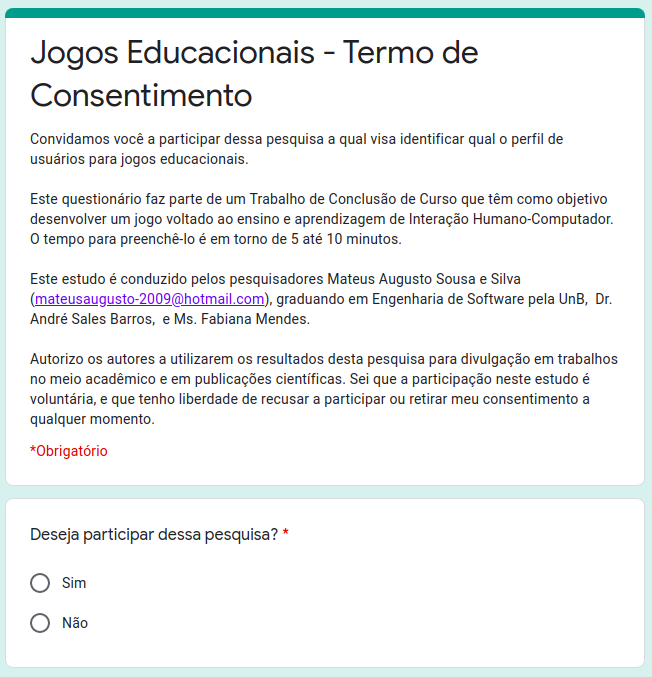
\includegraphics[keepaspectratio=true,scale=1.25]{figuras/apendice/survey1.png}
        \label{Fig:survey_pt1.png}
    }
    \quad
    \subfigure[Questionário Parte 2]{
        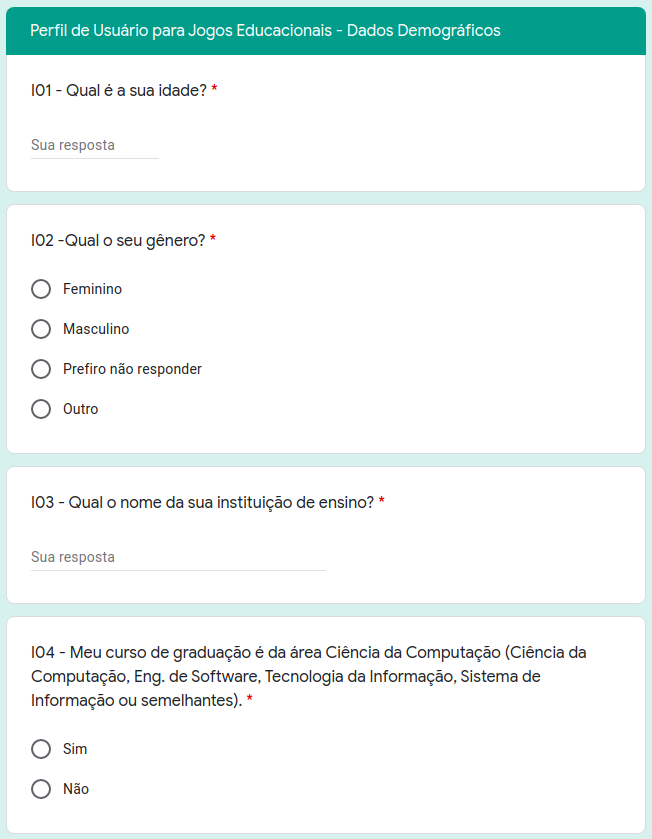
\includegraphics[keepaspectratio=true,scale=1.25]{figuras/apendice/survey2.png}
        \label{Fig:survey_pt2.png}
    }
    \quad
     \subfigure[Questionário Parte 3]{
        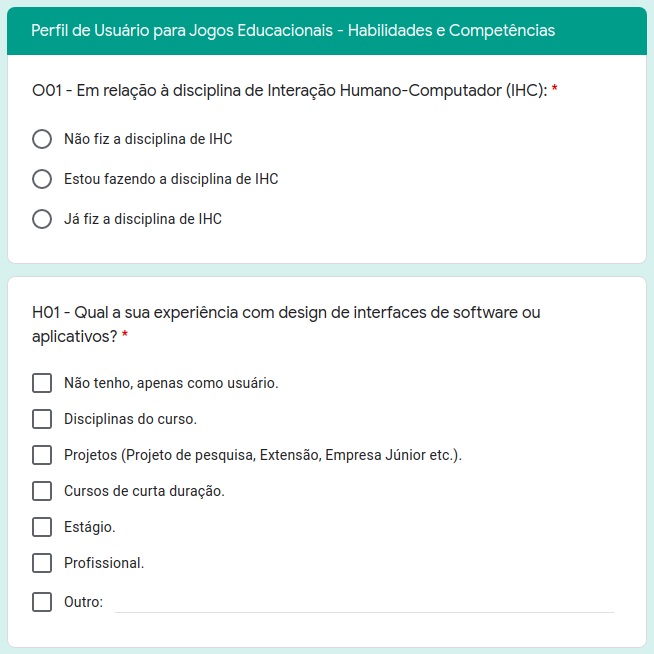
\includegraphics[keepaspectratio=true,scale=1.25]{figuras/apendice/survey3.png}
        \label{Fig:survey_pt3.png}
    }
    \quad
     \subfigure[Questionário Parte 4]{
        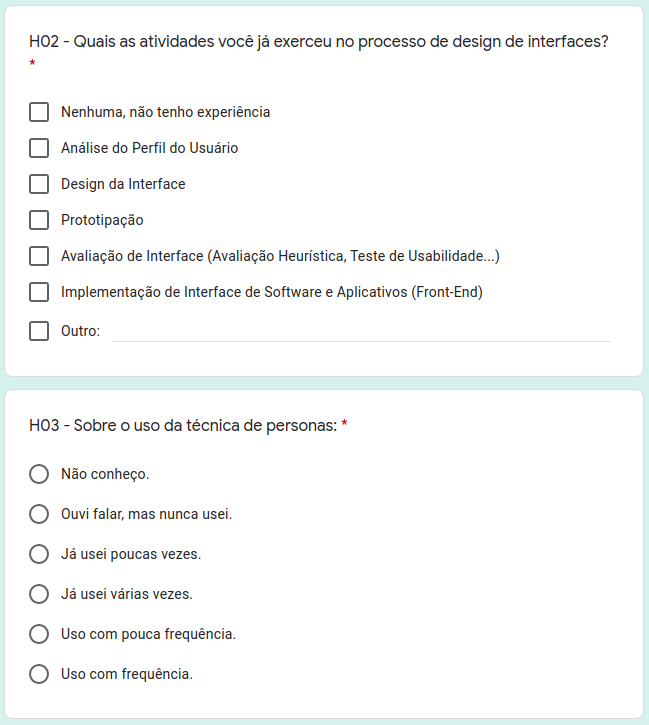
\includegraphics[keepaspectratio=true,scale=1.25]{figuras/apendice/survey4.png}
        \label{Fig:survey_pt4.png}
    }
   
	\caption{\textcolor{textmodified}{Questionário de Pesquisa 1-4 - Fonte: Mateus Augusto}}
	\label{Fig:survey1.png}
\end{figure}

\begin{figure}[htbp]
	\centering
	\subfigure[Questionário Parte 5]{
        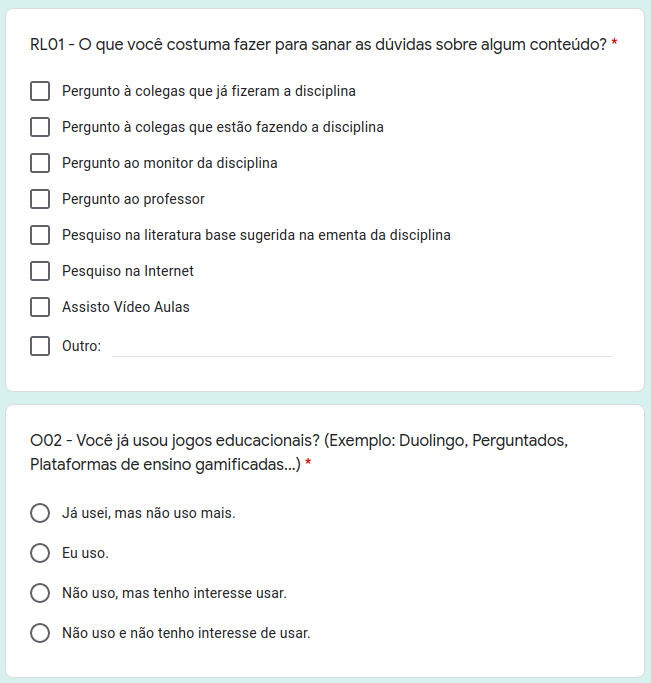
\includegraphics[keepaspectratio=true,scale=1.25]{figuras/apendice/survey5.png}
        \label{Fig:survey_pt5.png}
    }
    \quad
    \subfigure[Questionário Parte 6]{
        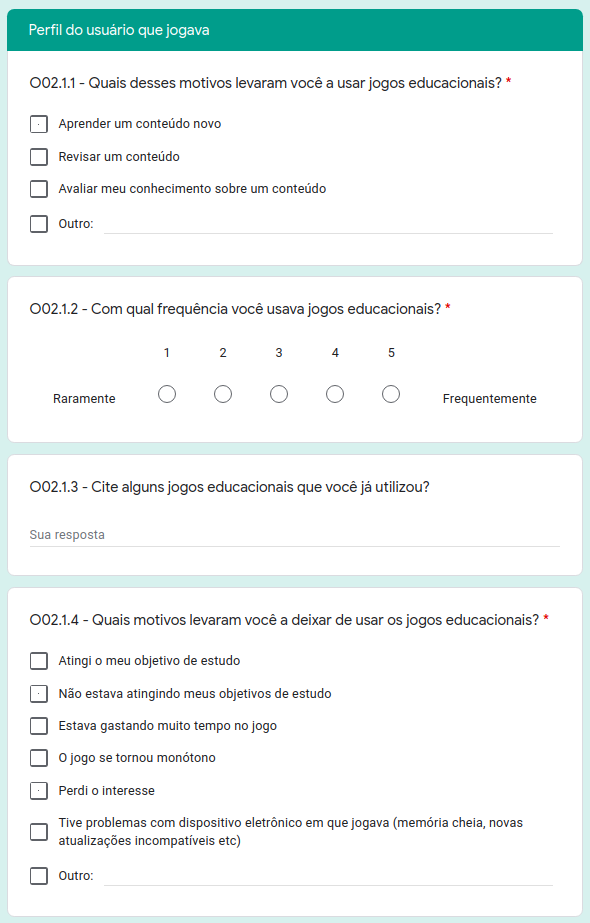
\includegraphics[keepaspectratio=true,scale=1.25]{figuras/apendice/survey6.png}
        \label{Fig:survey_pt6.png}
    }
    \quad
     \subfigure[Questionário Parte 7]{
        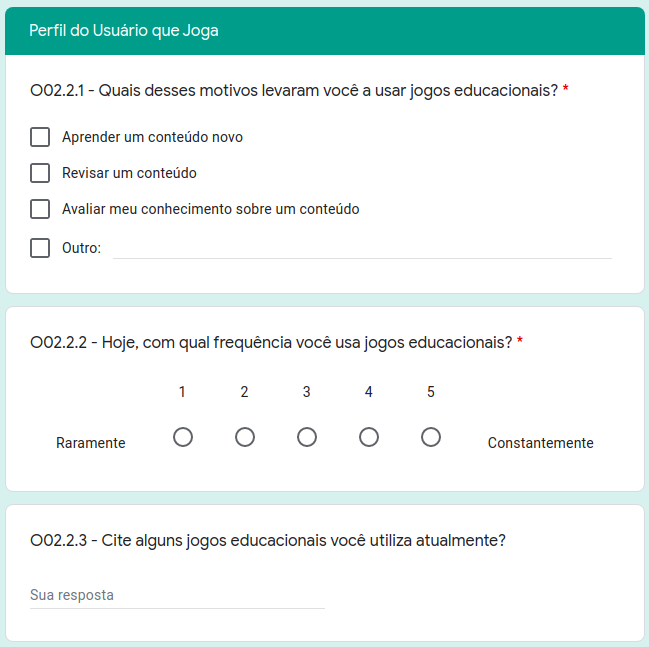
\includegraphics[keepaspectratio=true,scale=1.25]{figuras/apendice/survey7.png}
        \label{Fig:survey_pt7.png}
    }
    \quad
     \subfigure[Questionário Parte 8]{
        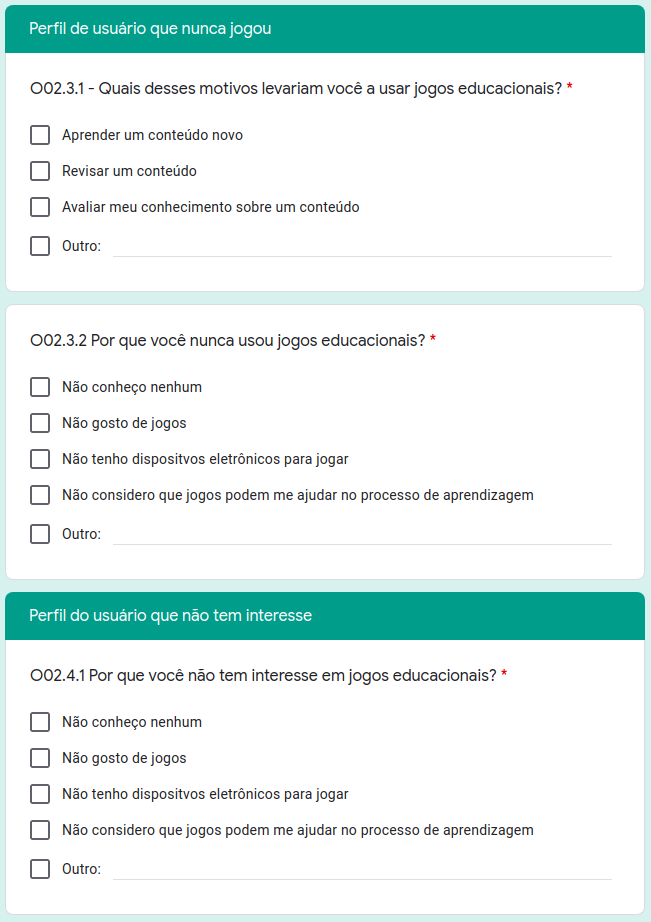
\includegraphics[keepaspectratio=true,scale=1.25]{figuras/apendice/survey8.png}
        \label{Fig:survey_pt8.png}
    }
   
	\caption{\textcolor{textmodified}{Questionário de Pesquisa 5-8 - Fonte: Mateus Augusto}}
	\label{Fig:survey2.png}
\end{figure}

\begin{figure}[htbp]
	\centering
	\subfigure[Questionário Parte 9]{
        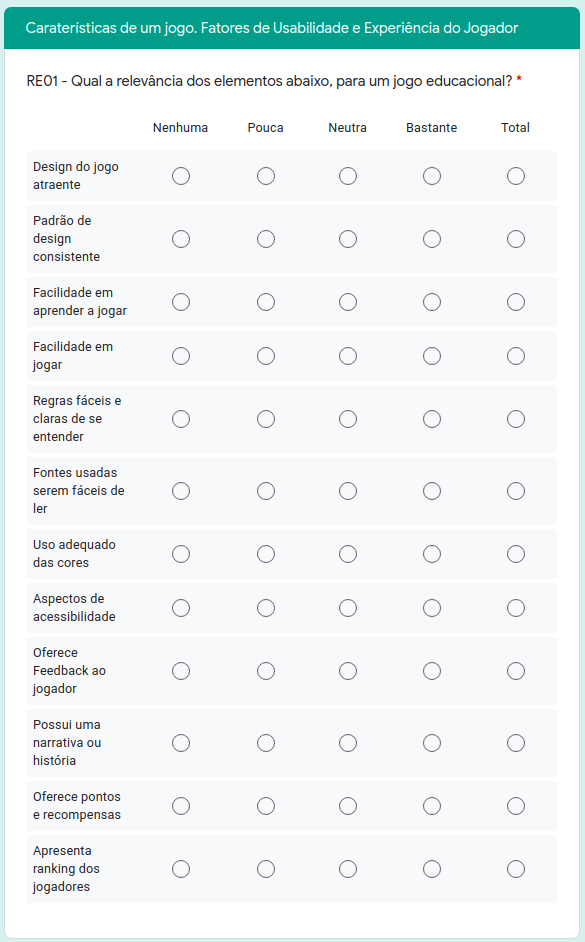
\includegraphics[keepaspectratio=true,scale=1.25]{figuras/apendice/survey9.png}
        \label{Fig:survey_pt9.png}
    }
    \quad
    \subfigure[Questionário Parte 10]{
        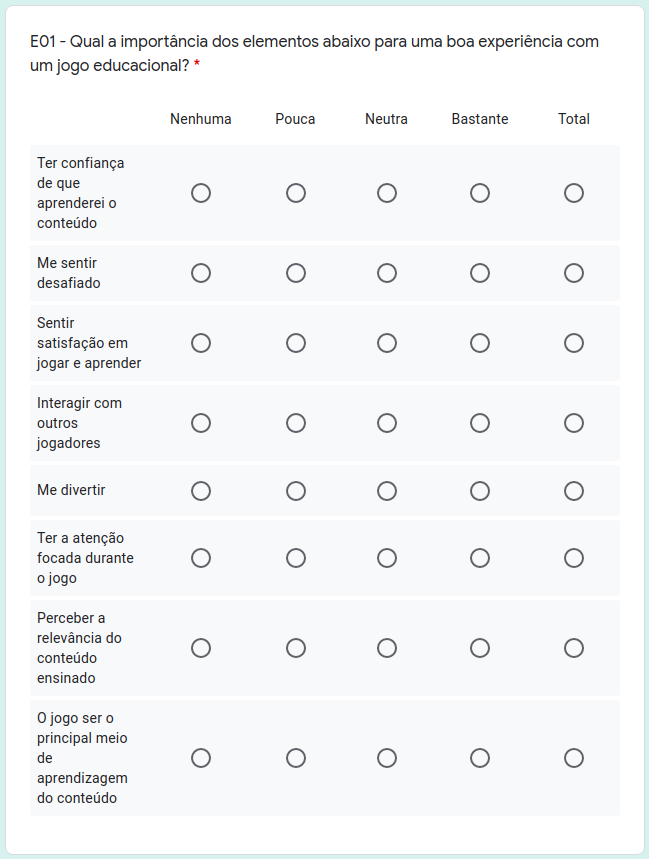
\includegraphics[keepaspectratio=true,scale=1.25]{figuras/apendice/survey10.png}
        \label{Fig:survey_pt10.png}
    }
    \quad
     \subfigure[Questionário Parte 11]{
        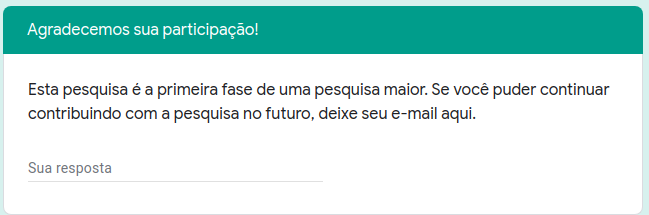
\includegraphics[keepaspectratio=true,scale=1.25]{figuras/apendice/survey11.png}
        \label{Fig:survey_pt11.png}
    }
   
	\caption{\textcolor{textmodified}{Questionário de Pesquisa 9-11 - Fonte: Mateus Augusto}}
	\label{Fig:survey3.png}
\end{figure}

\chapter{Relatório de Execução e Resultados do Questionário de Pesquisa}
\label{ap:res_quest}

O objetivo deste \textit{Survey} foi de identificar o perfil de usuários e levantar requisitos para o jogo proposto neste trabalho. Como o foco deste estudo é voltado para o desenvolvimento de um jogo que auxilie o ensino da técnica de Personas, o público-alvo, a quem foi direcionado o questionário, foram alunos de graduação e pós-graduação de cursos da área de Ciência da Computação. Foi planejado para este estudo, um período de quatro semanas para a coleta dos dados, ou seja, a amostra de pesquisa foram os respondentes do dia 06/10/2020 ao dia 27/10/2020. 

As perguntas do questionário foram elaboradas baseando-se na literatura revista. Foram usadas como base as características do modelo de personas em "\citeauthor{usability2020}", os atributos das personas descritas por \citeonline[p. 177]{barbosa_silva}, as características de jogos sérios em IHC identificados por \citeonline{deSales_SousaeSilva_2020} e as metas de usabilidade e experiência do jogador descritas por \citeonline{Petri_Wangenheim_2019}. Na Tabela \ref{tab:Table_survey} são apresentados os objetivos de cada questão, apontado por seu identificador (ID) no questionário, a referencia da figura onde é apresentada a questão e a base de onde foi elaborada a pergunta.

%longtable

\begin{table}[ht]
\centering
\caption{Rastreabilidade do Questionário}
\label{tab:Table_survey}
\begin{tabular}{|l|l|l|}
\hline
\textbf{ID} & \textbf{Objetivos}                                              & \textbf{Origem}   \\ \hline
I01         & - Usar como base para caracterização das personas               & UG, HC            \\ \hline
I02         & - Usar como base para caracterização das personas               & UG, HC            \\ \hline
I03         & - Usar como base para caracterização das personas               & UG, HC            \\ \hline
I04         & \begin{tabular}[c]{@{}l@{}}
              - Usar como base para caracterização das personas.\\ 
              - Controlar se respondente se enquadra no perfil do público-alvo
              \end{tabular}                                                   & UG, HC            \\ \hline
O01         & \begin{tabular}[c]{@{}l@{}}
              - Auxiliar na identificação dos objetivos das personas \\ 
              - Identificar o nível de conhecimento das personas
              \end{tabular}                                                   & UG, HC            \\ \hline
H01         & \begin{tabular}[c]{@{}l@{}}- Identificar o nível de conhecimento das personas \\ 
              - identificar as habilidades das personas
              \end{tabular}                                                   & UG, HC            \\ \hline
H02         & \begin{tabular}[c]{@{}l@{}}
              - Identificar o nível de conhecimento das personas \\ 
              - identificar as habilidades das personas
              \end{tabular}                                                 & UG, HC              \\ \hline
H03         & \begin{tabular}[c]{@{}l@{}} 
              - Auxiliar na validação da oportunidade de intervenção proposta\\ neste trabalho.
              \end{tabular} & UG, HC                                                              \\ \hline
RL01        & - Identificar com quem a persona se relaciona                   & HC                \\ \hline
O02         & \begin{tabular}[c]{@{}l@{}} 
              - Auxiliar na identificação dos objetivos das personas   \\       
              - Auxiliar na validação da oportunidade de intervenção proposta\\ neste trabalho.
              \end{tabular} & UG, HC            \\ \hline
O02.1.1     & - Identificar objetivos das personas                            & UG, HC            \\ \hline
O02.1.2     & \begin{tabular}[c]{@{}l@{}}
              - Auxiliar na identificação dos objetivos das personas\\ 
              - Identificar característica da tarefa realizada pela persona
              \end{tabular}                                                   & UG, HC            \\ \hline
O02.1.3     & - Usar como base para levantamento de alguns requisitos         &   -               \\ \hline
O02.1.4     & - Auxiliar na identificação dos objetivos das personas          & UG, HC            \\ \hline
O02.2.1     & - Identificar objetivos das personas                            & UG, HC            \\ \hline
O02.2.2     & \begin{tabular}[c]{@{}l@{}}
              - Auxiliar na identificação dos objetivos das personas\\ 
              - Identificar característica da tarefa realizada pela persona
              \end{tabular}                                                   & UG, HC            \\ \hline
O02.2.3     & - Usar como base para levantamento de alguns requisitos         &   -               \\ \hline
O02.3.1     & - Identificar objetivos das personas                            & UG, HC            \\ \hline
O02.3.2     & - Auxiliar na identificação dos objetivos das personas                    & UG, HC  \\ \hline
O02.4.1     & - Auxiliar na identificação dos objetivos das personas                    & UG, HC  \\ \hline
RE01        & - Identificar requisitos para o jogo                                      & \begin{tabular}[c]{@{}l@{}}
                                                                                          UG, HC, \\ 
                                                                                          JS, ME
                                                                                         \end{tabular}  \\ \hline
E01         & \begin{tabular}[c]{@{}l@{}}
              - Identificar requisitos para o jogo\\ 
              - Definir as metas de experiência do jogador\end{tabular}                & \begin{tabular}[c]{@{}l@{}}
                                                                                          UG, HC, \\ 
                                                                                          JS, ME
                                                                                         \end{tabular}  \\ \hline
\multicolumn{3}{p{15cm}}{\textbf{Legenda:} UG - \citeonline{usability2020}; HC - \citeonline{barbosa_silva} ; JS - \citeonline{deSales_SousaeSilva_2020}; ME - \citeonline{Petri_Wangenheim_2019}} \\
\end{tabular}
\end{table}

Antes da distribuição do questionário foi realizado um teste piloto com três pessoas. O objetivo do teste foi coletar \textit{feedbacks} sobre a compreensão e o \textit{layout} das perguntas, a estrutura e o fluxo do questionário e também identificar erros e o tempo médio para finalizar o questionário. O teste piloto foi realizado virtualmente, via plataforma de vídeo-chamada. Primeiramente o respondente recebeu algumas informações introdutórias sobre a pesquisa, em seguida ele acessou o questionário em seu computador e ativou o compartilhamento de tela. Dada a confirmação para o início da execução do questionário foram anotadas as percepções do avaliador enquanto o participante respondia. Concluído o teste piloto, foram anotados pelo avaliador, o relato oral dos respontes sobre suas percepções ao longo da execução do questionário. Depois de analisadas as anotações, foram aplicadas as sugestões de melhoria e corrigidos os erros encontrados no questionário. 

Em sua versão final, o questionário foi distribuído via meios de comunicação virtuais (mensagens de e-mail e em redes sociais), para a comunidade discente das instituições de ensino da Universidade de Brasília (UnB), Universidade Federal do Mato Grosso do Sul (UFMS), Universidade Federal do Amazonas (UFAM), Universidade Federal do Mato Grosso (UFMT) e Universidade Católica de Salvador (UCSAL). O questionário completo se encontra na seção de Apêndice \ref{ap:questionario}. 

% Apresentar fluxo e bifurcação das perguntas do questionário

Foram coletados os registros de 184 respondentes. Destes, foram identificados pelos endereços de e-mail fornecidos, que houveram 8 pessoas que responderam ao questionário mais de uma vez. Neste caso foi considerada válida apenas o último registro, sendo que as demais foram descartadas, permanecendo 176 registros. Foram ainda retirados mais 10 respondentes, por não se tratarem de pessoas que cursaram graduação em ciência da computação, restando por fim 166 registros. 
 
Dos respondentes, 128 são do sexo Masculino e 36 Feminino. Pode-se identificar que 1 respondente se declarou como de Outro sexo e 1 preferiu não responder. Segue a Figura \ref{Fig:genero.png}, dos sexos dos respondentes.

\begin{figure}[htbp]
	\centering
	\caption{Sexo dos respondentes}
	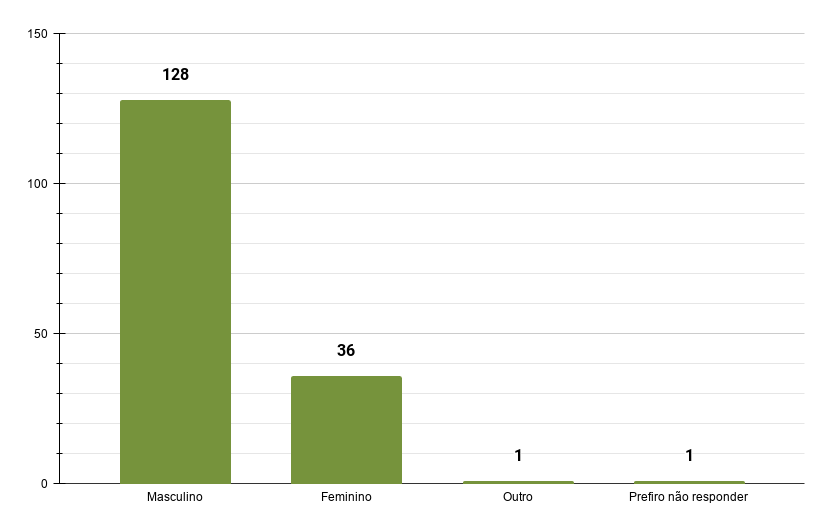
\includegraphics[keepaspectratio=true,scale=0.54]{figuras/apendice/graficos_survey/genero.png}
	\label{Fig:genero.png}
\end{figure}

Em relação à idade dos respondentes foi observado que a idade mínima foi de 18 anos e a máxima de 53 anos, sendo que 75\% deles é composto por jovens de até 23 anos de idade. A idade mais frequente foi a de 21 anos, com 29 respondentes. Não houveram respondentes com idades de 29, 33, 34, 37, 39, 41, 42, 43, 44, 45, 46, 48, 49, 50, 51 e 52 anos. A Figura \ref{Fig:idade.png}, da idade dos respondentes.

\newpage
\begin{figure}[htbp]
	\centering
	\caption{Relação da quantidade de respondentes por idade}
	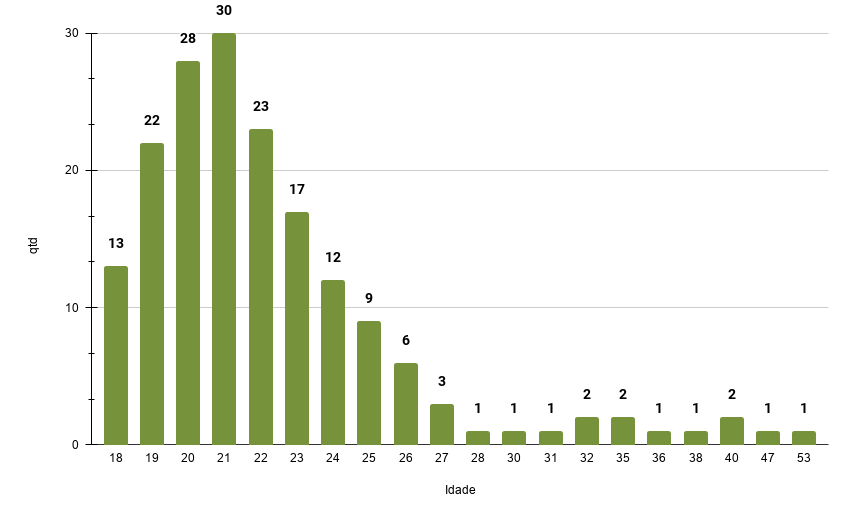
\includegraphics[keepaspectratio=true,scale=0.51]{figuras/apendice/graficos_survey/idade.png}
	\label{Fig:idade.png}
\end{figure}

Dentre as instituições de ensino que participaram da pesquisa, foram obtidas 126 respostas na UnB, 24 na UFMS, 10 na UFAM, 4 na UFMT, 1 resposta na UCSAL e UTFPR, cada e 0 respostas na UFU. A Figura \ref{Fig:campus.png}, dos Instituições de ensino.

\begin{figure}[htbp]
	\centering
	\caption{Instituições de ensino dos respondentes}
	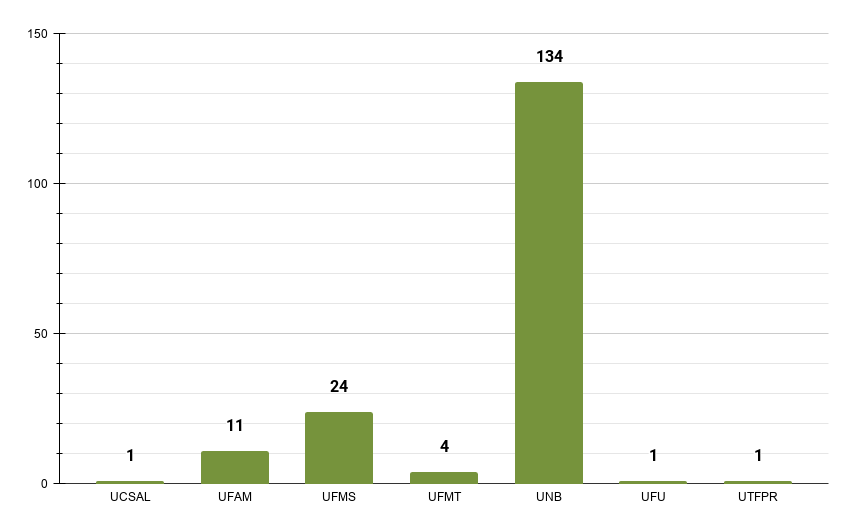
\includegraphics[keepaspectratio=true,scale=0.5]{figuras/apendice/graficos_survey/campus.png}
	\label{Fig:campus.png}
\end{figure}

\newpage
Em relação aos respondentes e o curso de Interação Humano-Computador, foi observado que 44 respondentes não haviam feito a disciplina, 26,5\% do total; 57 já haviam feito a disciplina, 34,3\% do total; e 65 estavam fazendo a disciplina durante esta pesquisa, 39,2\% do total. A Figura \ref{Fig:curso.png}, da relação dos respondentes e o curso de IHC.

\begin{figure}[htbp]
	\centering
	\caption{Relação do respondente com o curso de IHC}
	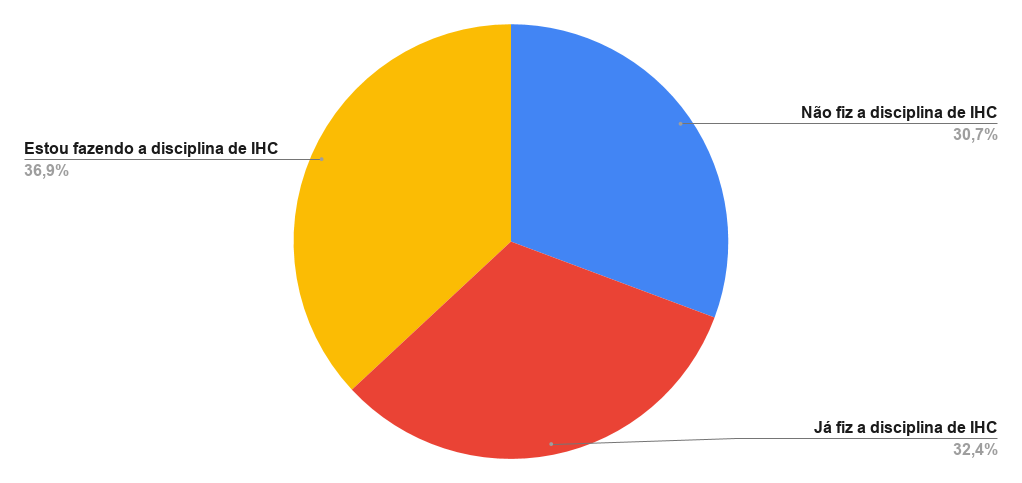
\includegraphics[keepaspectratio=true,scale=0.4]{figuras/apendice/graficos_survey/curso.png}
	\label{Fig:curso.png}
\end{figure}
    
\chapter{Relatório de Execução e Resultados da Construção as Personas}
\label{ap:persona}

{\color{textmodified}
Neste capítulo de apêndice é apresentado o relatório de execução e os resultados do processo de construção das personas deste trabalho. A partir dos dados dos respondentes do questionário de pesquisa do \textit{Survey}, apresentado no Apêndice \ref{ap:res_quest} foi possível definir o elenco de personas deste projeto. Na Figura \ref{Fig:process_persona.png} é demonstrada uma visão geral das etapas para a definição das personas.
}

\begin{figure}[htbp]
	\centering
	\caption{Processo de Construção das personas}
	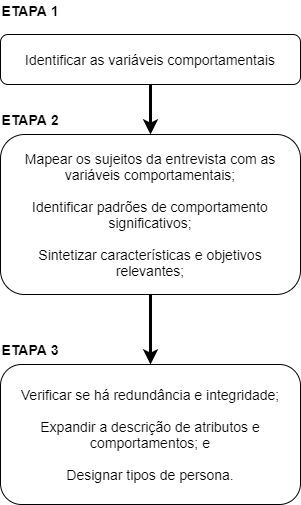
\includegraphics[keepaspectratio=true,scale=0.8]{figuras/personas/process_persona.png}
	\label{Fig:process_persona.png}
\end{figure}

Na primeira etapa foram identificadas as variáveis comportamentais. Estas foram definidas a partir das respostas provenientes do próprio questionário de pesquisa, registradas em uma planilha eletrônica (PE0). Seguem as variáveis:

\begin{itemize}
    \item I01, I02 e I03 (\ref{Fig:survey_pt2.png}): complementa a caracterização da persona, dando aspectos mais reais a ela;
    \item I04(\ref{Fig:survey_pt2.png}): pode evidenciar um certo grau de conhecimento mais técnico entre os usuários que cursam graduação na área de Ciência da Computação e os de outros cursos;
    \item O01(\ref{Fig:survey_pt3.png}): pode evidenciar um certo grau de conhecimento e experiência do usuário em relação a área de Interação Humano-Computador;
    \item H01(\ref{Fig:survey_pt3.png}): pode evidenciar um certo grau de conhecimento e experiência mais prática em IHC;
    \item H02(\ref{Fig:survey_pt4.png}): pode evidenciar um certo grau de conhecimento e experiência mais prática em IHC;
    \item RL01(\ref{Fig:survey_pt5.png}): ajuda a apontar os relacionamentos mais relevantes do usuário no contexto de ensino e aprendizagem, que serve para identificar uma oportunidade de intervenção em que um jogo educacional pode auxiliar nessas relações;
    \item O02(\ref{Fig:survey_pt5.png}): quesito base que evidencia o nível de afinidade do usuário com jogos educacionais;
    \item O02.1.1(\ref{Fig:survey_pt6.png}), O02.2.1(\ref{Fig:survey_pt7.png}) e O02.3.1(\ref{Fig:survey_pt8.png}): quesito que evidencia o objetivo do usuário ao usar um jogo educacional;
    \item O02.1.2(\ref{Fig:survey_pt6.png}) e O02.2.2(\ref{Fig:survey_pt7.png}): auxilia na percepção da frequência em que os usuários costumam usar jogos educacionais;
    \item O02.1.4(\ref{Fig:survey_pt6.png}): auxilia na identificação de usuários específicos que têm uma afinidade relevante para com os jogos educacionais; 
    \item O02.3.2(\ref{Fig:survey_pt8.png}) e O02.4.1(\ref{Fig:survey_pt8.png}): auxilia na complementação das características das anti-personas
    \item RE01(\ref{Fig:survey_pt9.png}) e E01(\ref{Fig:survey_pt10.png}): serve para identificar a preferencia dos usuários em relação às características e experiências dos jogos educacionais;
\end{itemize}

Após a identificação das variáveis comportamentais o passo seguinte foi o mapeamento dos respondentes em relação a essas variáveis, a identificação de padrões de comportamento significativos e a sintetização de características e objetivos relevantes. Essas três etapas foram executadas de forma simultânea até ser possível ter as estruturas base das personas. 

Como as respostas do questionário foram armazenadas em uma planilha eletrônica (PE0), fez-se uso desta ferramenta para a filtragem e síntese dos dados. Primeiramente foram divididas em duas planilhas os dados dos respondentes a partir da variável I04. Definindo então a estrutura base da anti-persona (PE2), aqueles que não são da área de Ciência da Computação, e também a estrutura das demais personas (PE1). Na Figura \ref{Fig:persona_tree.png} é apresentada o processo de refino das planilhas para a construção das personas.

\begin{figure}[htbp]
	\centering
	\caption{Fluxo do processo de construção das personas}
	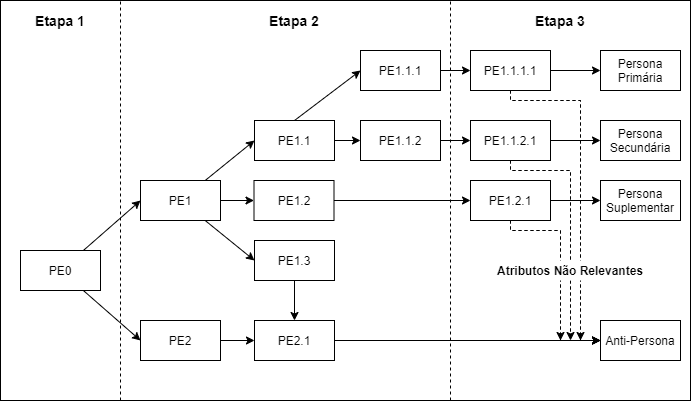
\includegraphics[keepaspectratio=true,scale=0.6]{figuras/personas/persona_tree.png}
	\label{Fig:persona_tree.png}
\end{figure}

Com a variável O02 foi possível possível separar 3 perfis a partir de PE1. Foram estes, o perfil daqueles que responderam que usavam jogos e os que já usaram, mas não jogavam mais (PE1.1); o perfil  daqueles que nunca jogaram, mas tinham um interesse (PE1.2); e o perfil daqueles que não tinham interesse de jogar (PE1.3), que no caso foi englobado ao PE2, formando o PE2.1.

Dentro de PE1.1 existiam aqueles que haviam jogado, mas por algum motivo tinham parado de usar jogos educacionais. Destes foram relevantes apenas aqueles que pararam de jogar por terem alcançado seu objetivo por meio do jogo. Foi obtido então PE1.1.1, com aqueles que jogam jogos educacionais e PE1.1.2, com aqueles que haviam jogado, mas pararam por haverem alcançado seu objetivo, estes foram identificados pela variável O02.1.4.

O próximo passo foi observar, a partir das variáveis H01, H02 e O01, quais os perfis seriam mais relevantes para o jogo devido ao padrão de comportamento expresso por esse grupo de variáveis. Foram definidos então os perfis na PE1.2.1, PE1.1.1.1 e PE1.1.2.1, cujo grupo comportamental expressava que o usuário tinha um conhecimento sobre IHC inicial ou nenhum conhecimento, sendo que estes ou estavam fazendo o curso de IHC ou ainda não haviam feito.

Tendo sido agrupados e filtrados esses conjuntos de características foi possível identificar os objetivos (O02.1.1, O02.2.1 e O02.3.1) dos jogadores. Primeiramente a busca por um jogo que auxilie no aprendizado de um conteúdo novo, depois um jogo que ajude na revisão de um conteúdo visto e a possibilidade de avaliar seu conhecimento através do jogo. Com os objetivos definidos, foi então identificada a experiência e elementos do jogos (RE01 e E01) mais relevantes buscados por cada perfil. % dá pra aprofundar mais nessa parte, mas nã é o foco do trabalho

Traçados esse esboço inicial dos perfis das personas, foi realizadas a última etapa. Foi verificada a integridade das personas e se haviam redundâncias, uma descrição mais detalhada de atributos e comportamentos foram inseridos tirando como base algumas variáveis comportamentais (RL01, O02.1.2 e O02.2.2) e outras variáveis de identificação (I01, I02 e I03). Por fim foram designados os tipos de personas, primária, secundária e suplementar. No caso da anti-persona, as variáveis O02.3.2 e O02.4.1 auxiliaram a complementar suas características, além dos atributos que foram considerados como irrelevantes para as outras personas.

A seguir encontram-se as personas construídas para esse projeto. A persona primária, Victor Matheus Farias (Tabela \ref{tab:Table_persona1}); a persona secundária, Afonso Souza de Queiroz (Tabela \ref{tab:Table_persona2}); a persona suplementar, Natália Figueiredo (Tabela \ref{tab:Table_persona3}); e a anti-persona, Rafael Medeiros (Tabela \ref{tab:Table_persona4}).
\newpage

\begin{table}[htbp]
\centering
\caption{Persona Primária}
\label{tab:Table_persona1}
\small
\begin{tabular}{| m{0.25\textwidth} m{0.65\textwidth}|}
\hline \multicolumn{2}{|c|}{\textbf{Identidade}} \\ \hline
& \\

\begin{center} 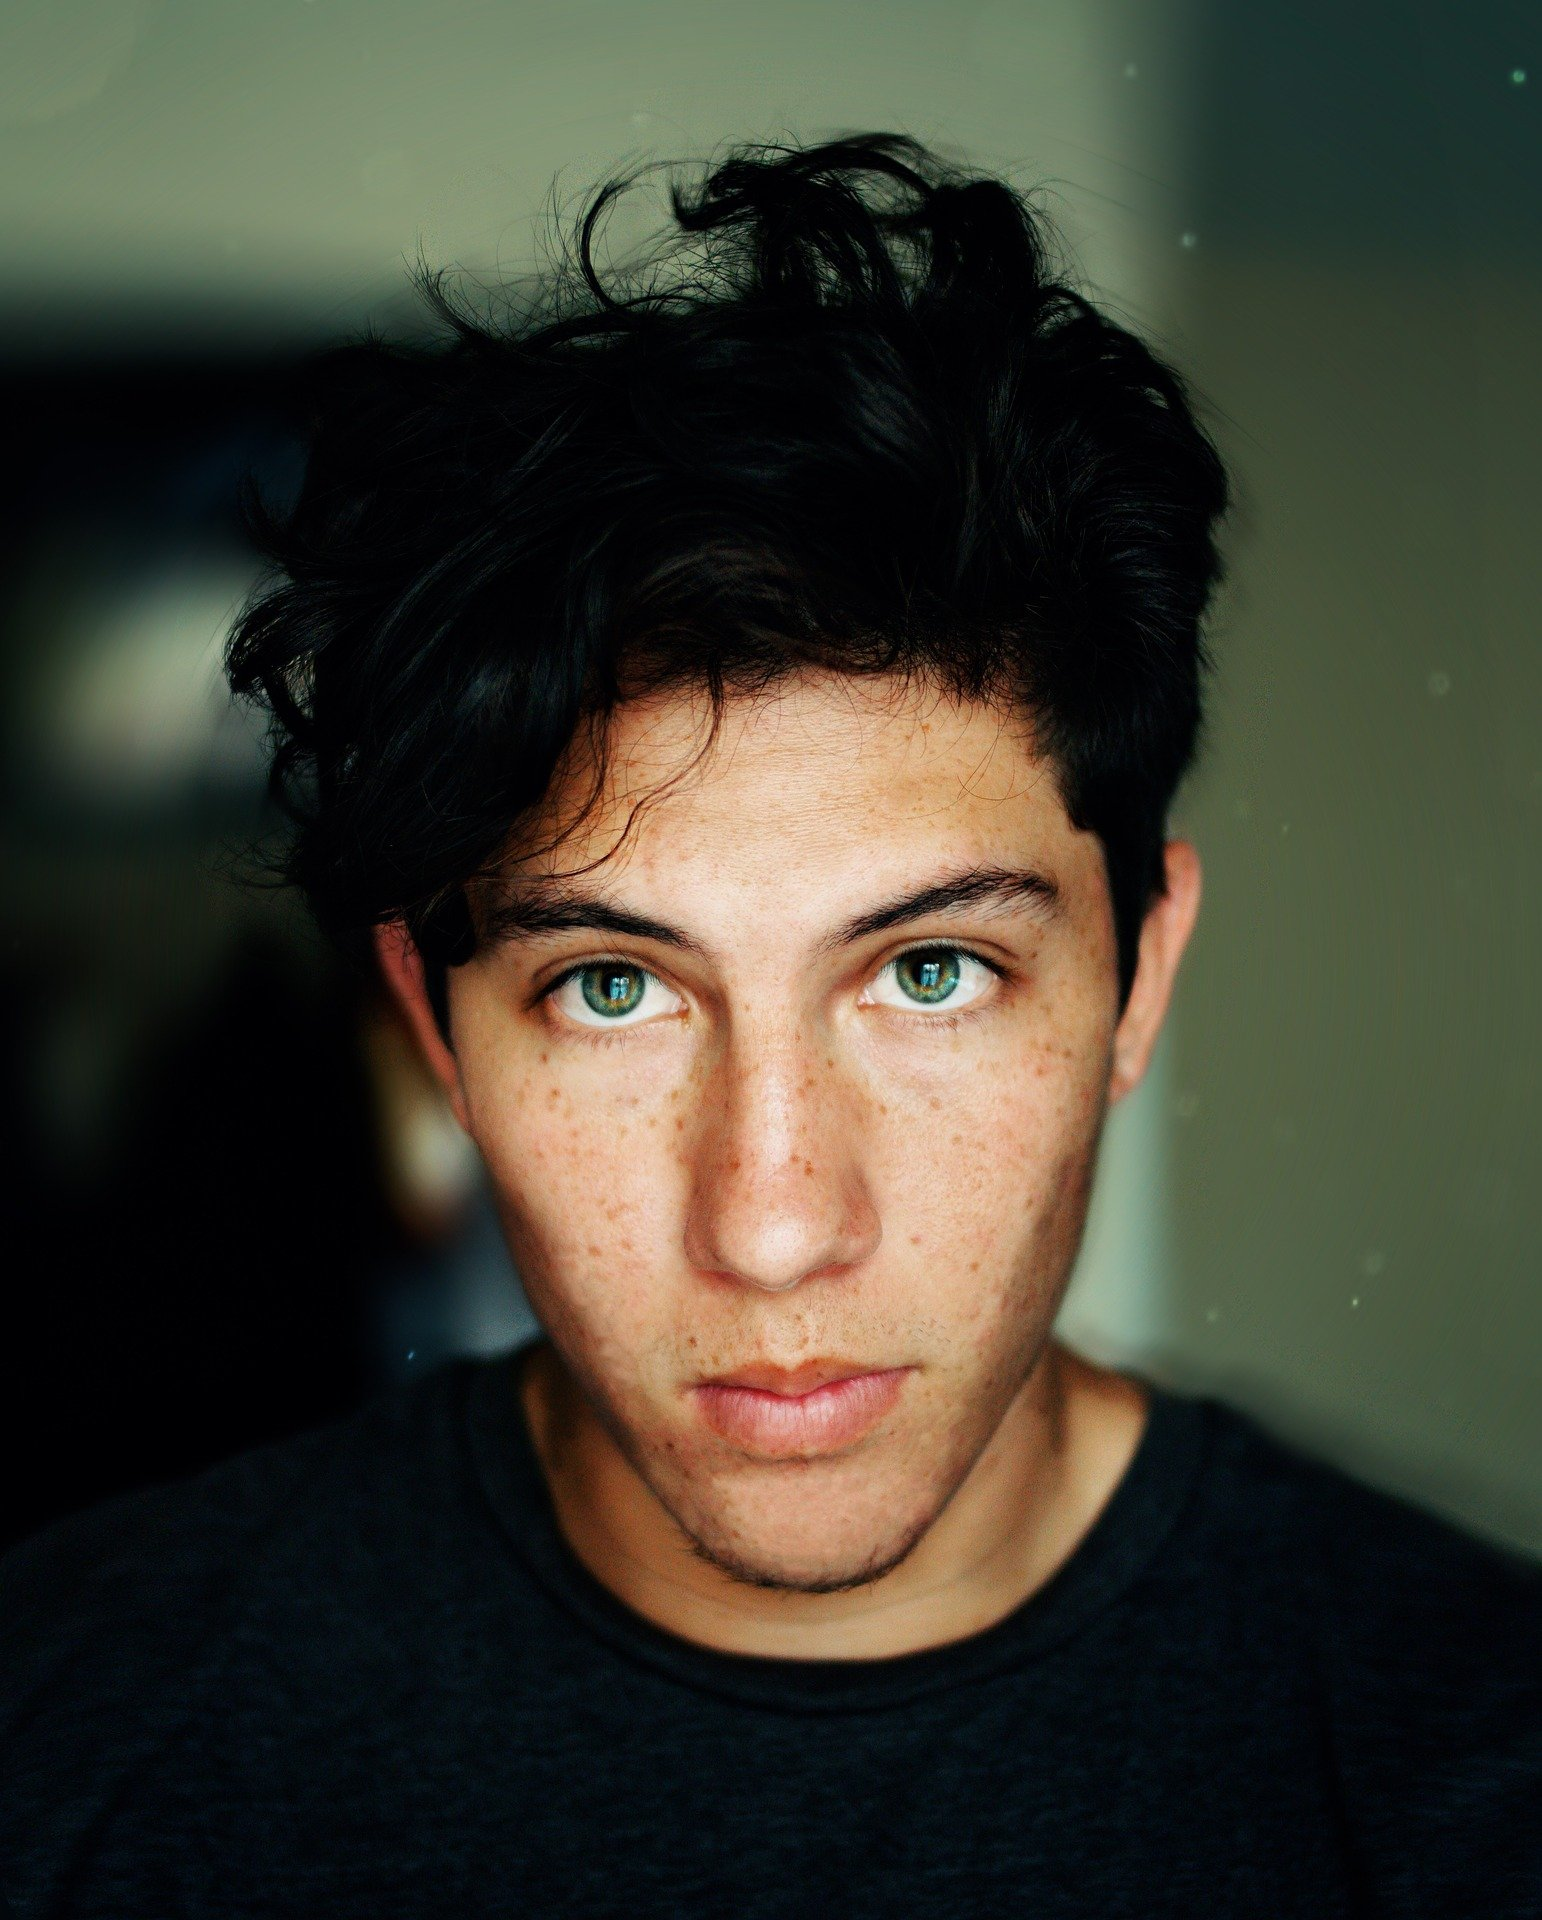
\includegraphics[scale=0.06]{figuras/personas/portrait-3353699_1920.jpg} \end{center} 

&

\textbf{Nome: } Victor Matheus Farias

\textbf{Idade:} 19 anos

\textbf{Ocupação:} Estudante de Engenharia de Software na UnB, Faculdade do Gama.

\\ \hline


\multicolumn{2}{|c|}{\textbf{Descrição}} \\ \hline
\multicolumn{2}{|p{15cm}|}{
        Aprender algum conteúdo novo é meu o principal objetivo ao usar jogos educacionais. Atualmente eu uso alguns jogos educacionais, mas com uma frequência moderada. Vejo-os como ferramentas que me auxiliam no processo de aprendizagem. Estou cursando a disciplina de IHC e não tenho muito conhecimento em relação a elaboração de design de interfaces e o pouco que tenho está somente no âmbito disciplinar, daquilo que já vi na disciplina. Desejaria utilizar um jogo que me ajudasse a aprender o conteúdo.
       
        Geralmente quando vou estudar ou sanar alguma dúvida que tenho sobre o conteúdo eu recorro primeiramente à artigos da internet. Em alguns casos assisto vídeo aulas e também utilizo do material disponibilizado pelo professor.
        
        Outros meios que uso para sanar as dúvidas que tenho em relação ao conteúdo é perguntar a colegas que já fizeram a disciplina e também geralmente estudo com colegas que estão fazendo a disciplina comigo. Busco em alguns casos tirar as dúvidas com os monitores ou professor.
        Os requisitos do jogo que me levam a usá-lo são: 
        \begin{itemize}
            \item um design atraente e consistente; 
            \item o jogo ser fácil de aprender a jogar e fácil de se jogar, com regras claras; 
            \item um bom uso de fontes e cores; 
            \item que o jogo ofereçam feedbacks relevantes. 
        \end{itemize}
        
        Ao usar um jogo eu espero ter certeza que vou  aprender o conteúdo ali apresentado, espero que seja algo desafiador, divertido e satisfatório aprender jogando. 
        
        Jogos que prendem minha atenção e me envolvem para aprender o conteúdo são bem relevantes, ainda mais se eu conseguir perceber a importância do conteúdo que estou aprendendo.} \\ \hline
\end{tabular}
\end{table}
\begin{table}[htbp]
\centering
\caption{Persona Secundária}
\label{tab:Table_persona2}
\small
\begin{tabular}{| m{0.25\textwidth} m{0.65\textwidth}|}
\hline \multicolumn{2}{|c|}{\textbf{Identidade}} \\ \hline
& \\

\begin{center} 
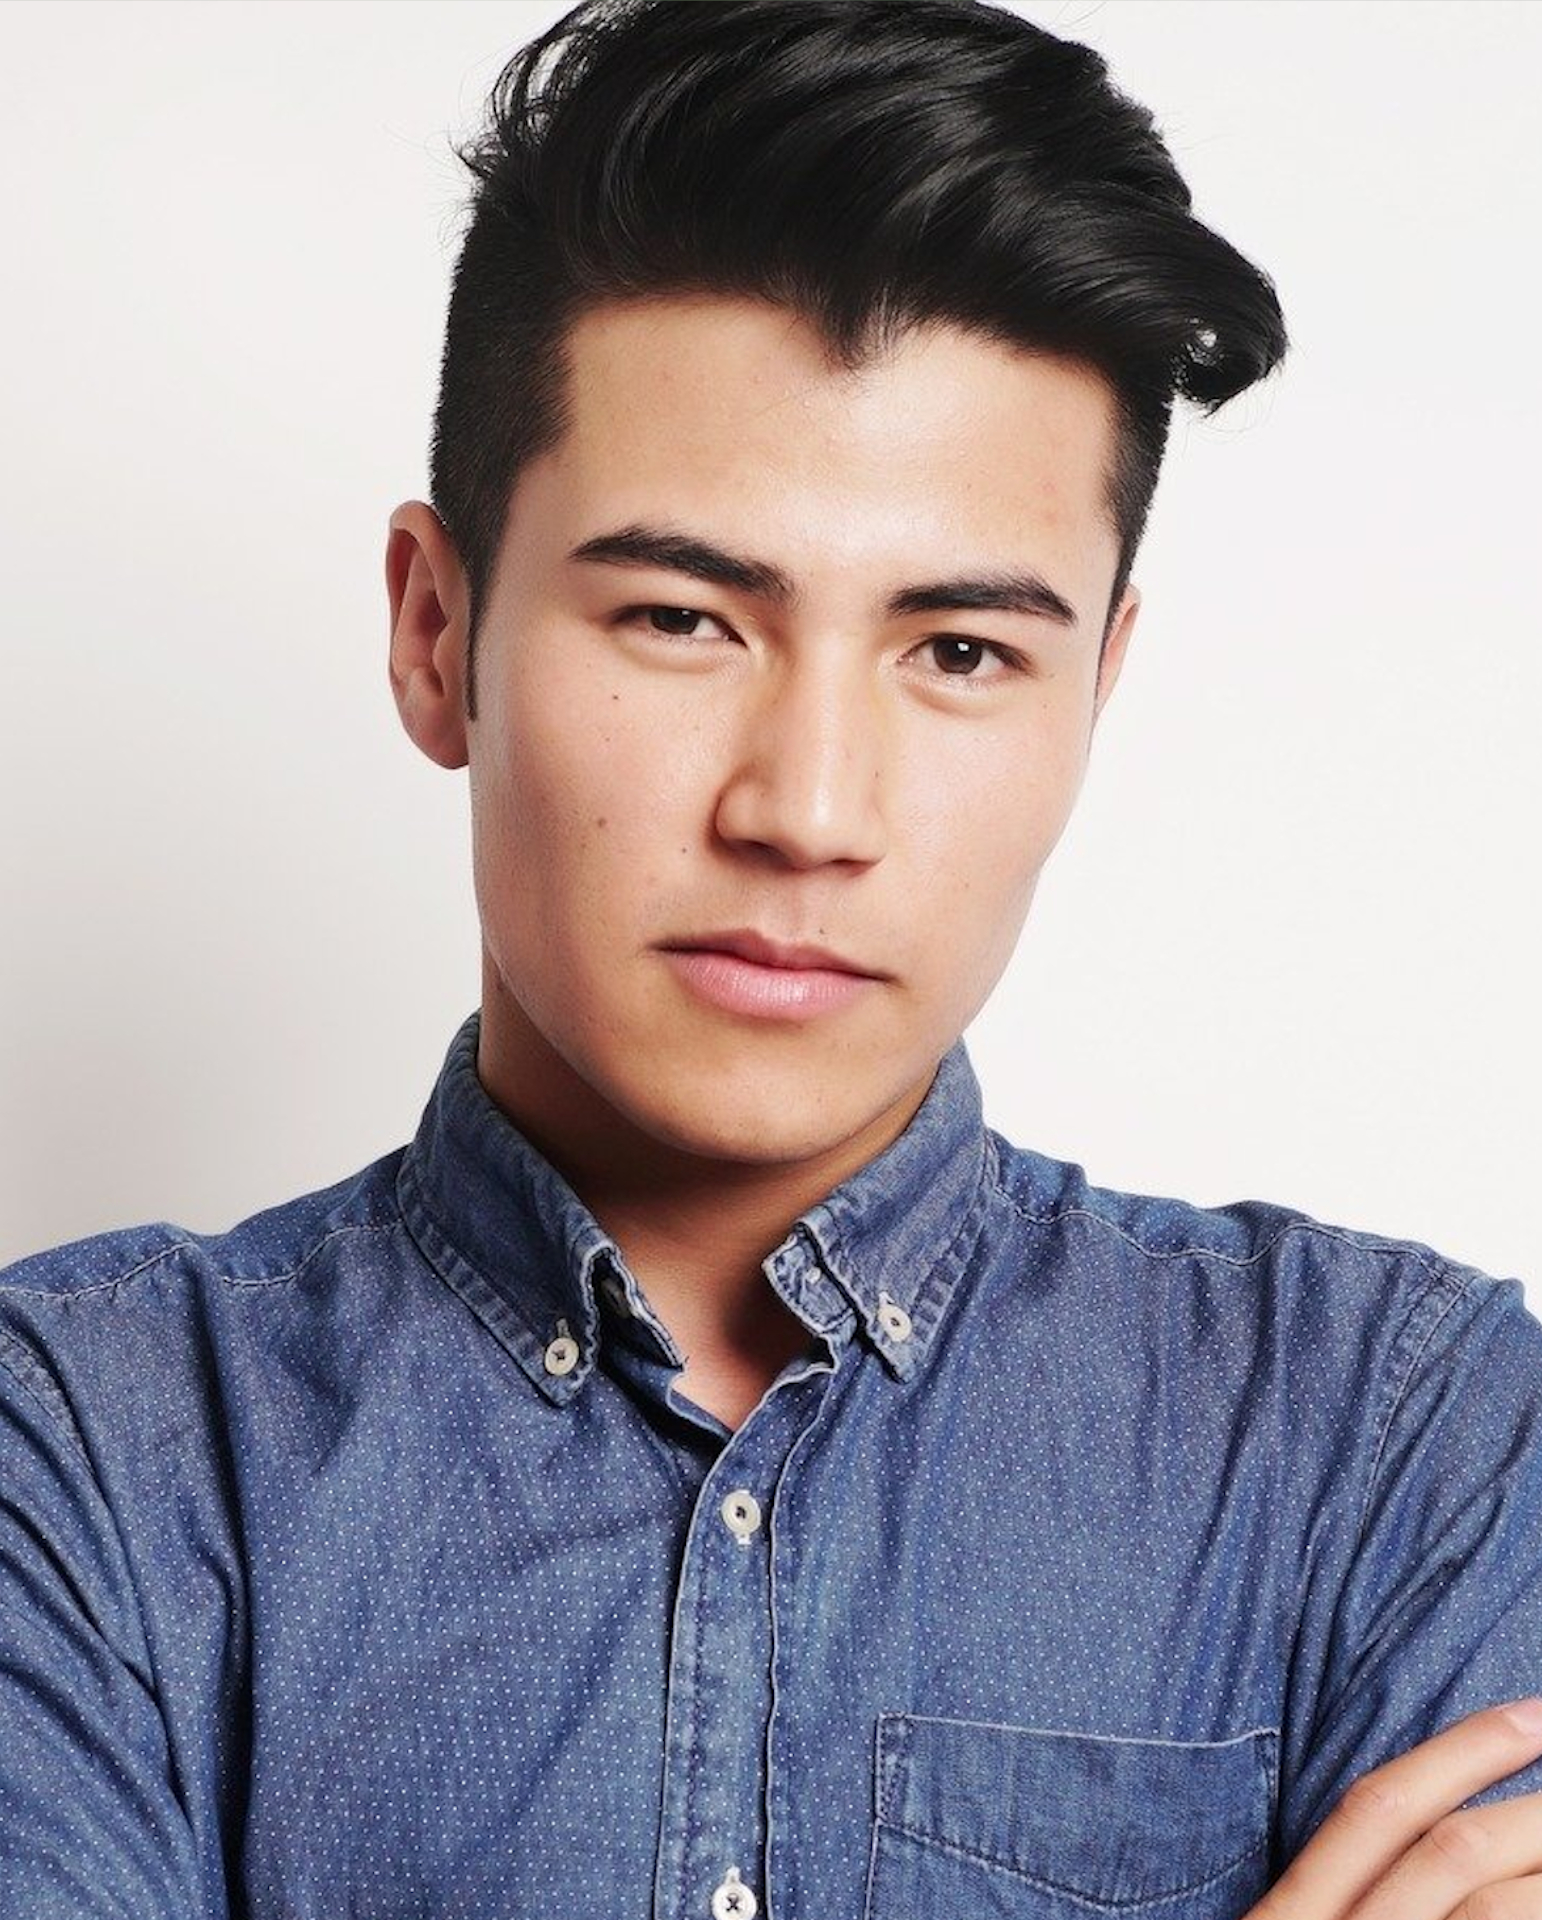
\includegraphics[scale=0.06]{figuras/personas/model-2911332_1920.jpg} 
Fonte: Pixabay\tablefootnote{https://pixabay.com/photos/model-businessman-corporate-2911332/}
\end{center} 

&

\textbf{Nome: } Afonso Souza de Queiroz

\textbf{Idade:} 19 anos

\textbf{Ocupação:} Estudante de Engenharia de Software na UnB, Faculdade do Gama

\\ \hline


\multicolumn{2}{|c|}{\textbf{Descrição}} \\ \hline
\multicolumn{2}{|p{15cm}|}{
     \begin{tabular}[c]{@{}l@{}}\\
        Já joguei alguns jogos educacionais onde meu principal objetivo era aprender um\\ conteúdo novo. Além disso era interessante quando o jogo possibilitava que eu revisasse\\ o conteúdo e avaliasse o que tinha aprendido. Eu jogava com certa moderação. Por mais\\ que atualmente eu não esteja usando algum jogo educacional, eu parei de jogar pois \\alcancei meus objetivos de estudo e me sentiria da mesma forma se houvesse algum\\ jogo que me ajudasse nas matérias da faculdade.\\ 
        \\
        Ainda não fiz a disciplina de IHC, por isso não tenho muito conhecimento em relação\\ a elaboração de design de interfaces, sendo que o pouco que tenho veio de projetos de\\ outras disciplinas e atividades extra curriculares.\\
        \\
        Gosto mais de estudar sozinho, pesquisando na internet e indo por conta própria atrás\\ de materiais de estudo. Apenas quando não acho nada relevante, recorro aos materiais\\ disponibilizados pelo professor.\\
        \\
        Para mim, um jogo onde vou aprender deve ter um design com um \textbf{padrão simples},\\ mas que desperte \textbf{interesse}; deve me dar bons \textbf{feedbacks} a cada interação que faço\\ no jogo; deve ser algo \textbf{simples de aprender como jogar} e \textbf{simples de jogar}; e caso\\ tenha textos sobre o conteúdo, seria bom que os textos fossem bem objetivos e com\\ uma cor e fonte que facilitasse a leitura.\\ 
        \\
        Espero ter a sensação logo de cara que \textbf{não vou perder meu tempo} com o jogo, mas\\ que ao final vou perceber o quanto foi \textbf{importante aprender o conteúdo} e o quanto\\ foi \textbf{satisfatório} ter me \textbf{divertido} aprendendo. E espero também de certa forma ser\\ \textbf{desafiado}, pois isso me ajuda a \textbf{focar} na atividade que estou realizando.\\ \\ 
    \end{tabular}
} \\ \hline
\end{tabular}
\end{table}
\newpage

\begin{table}[htbp]
\centering
\caption{Persona Suplementar}
\label{tab:Table_persona3}
\small
\begin{tabular}{| m{0.25\textwidth} m{0.65\textwidth}|}
\hline \multicolumn{2}{|c|}{\textbf{Identidade}} \\ \hline
& \\

\begin{center} 
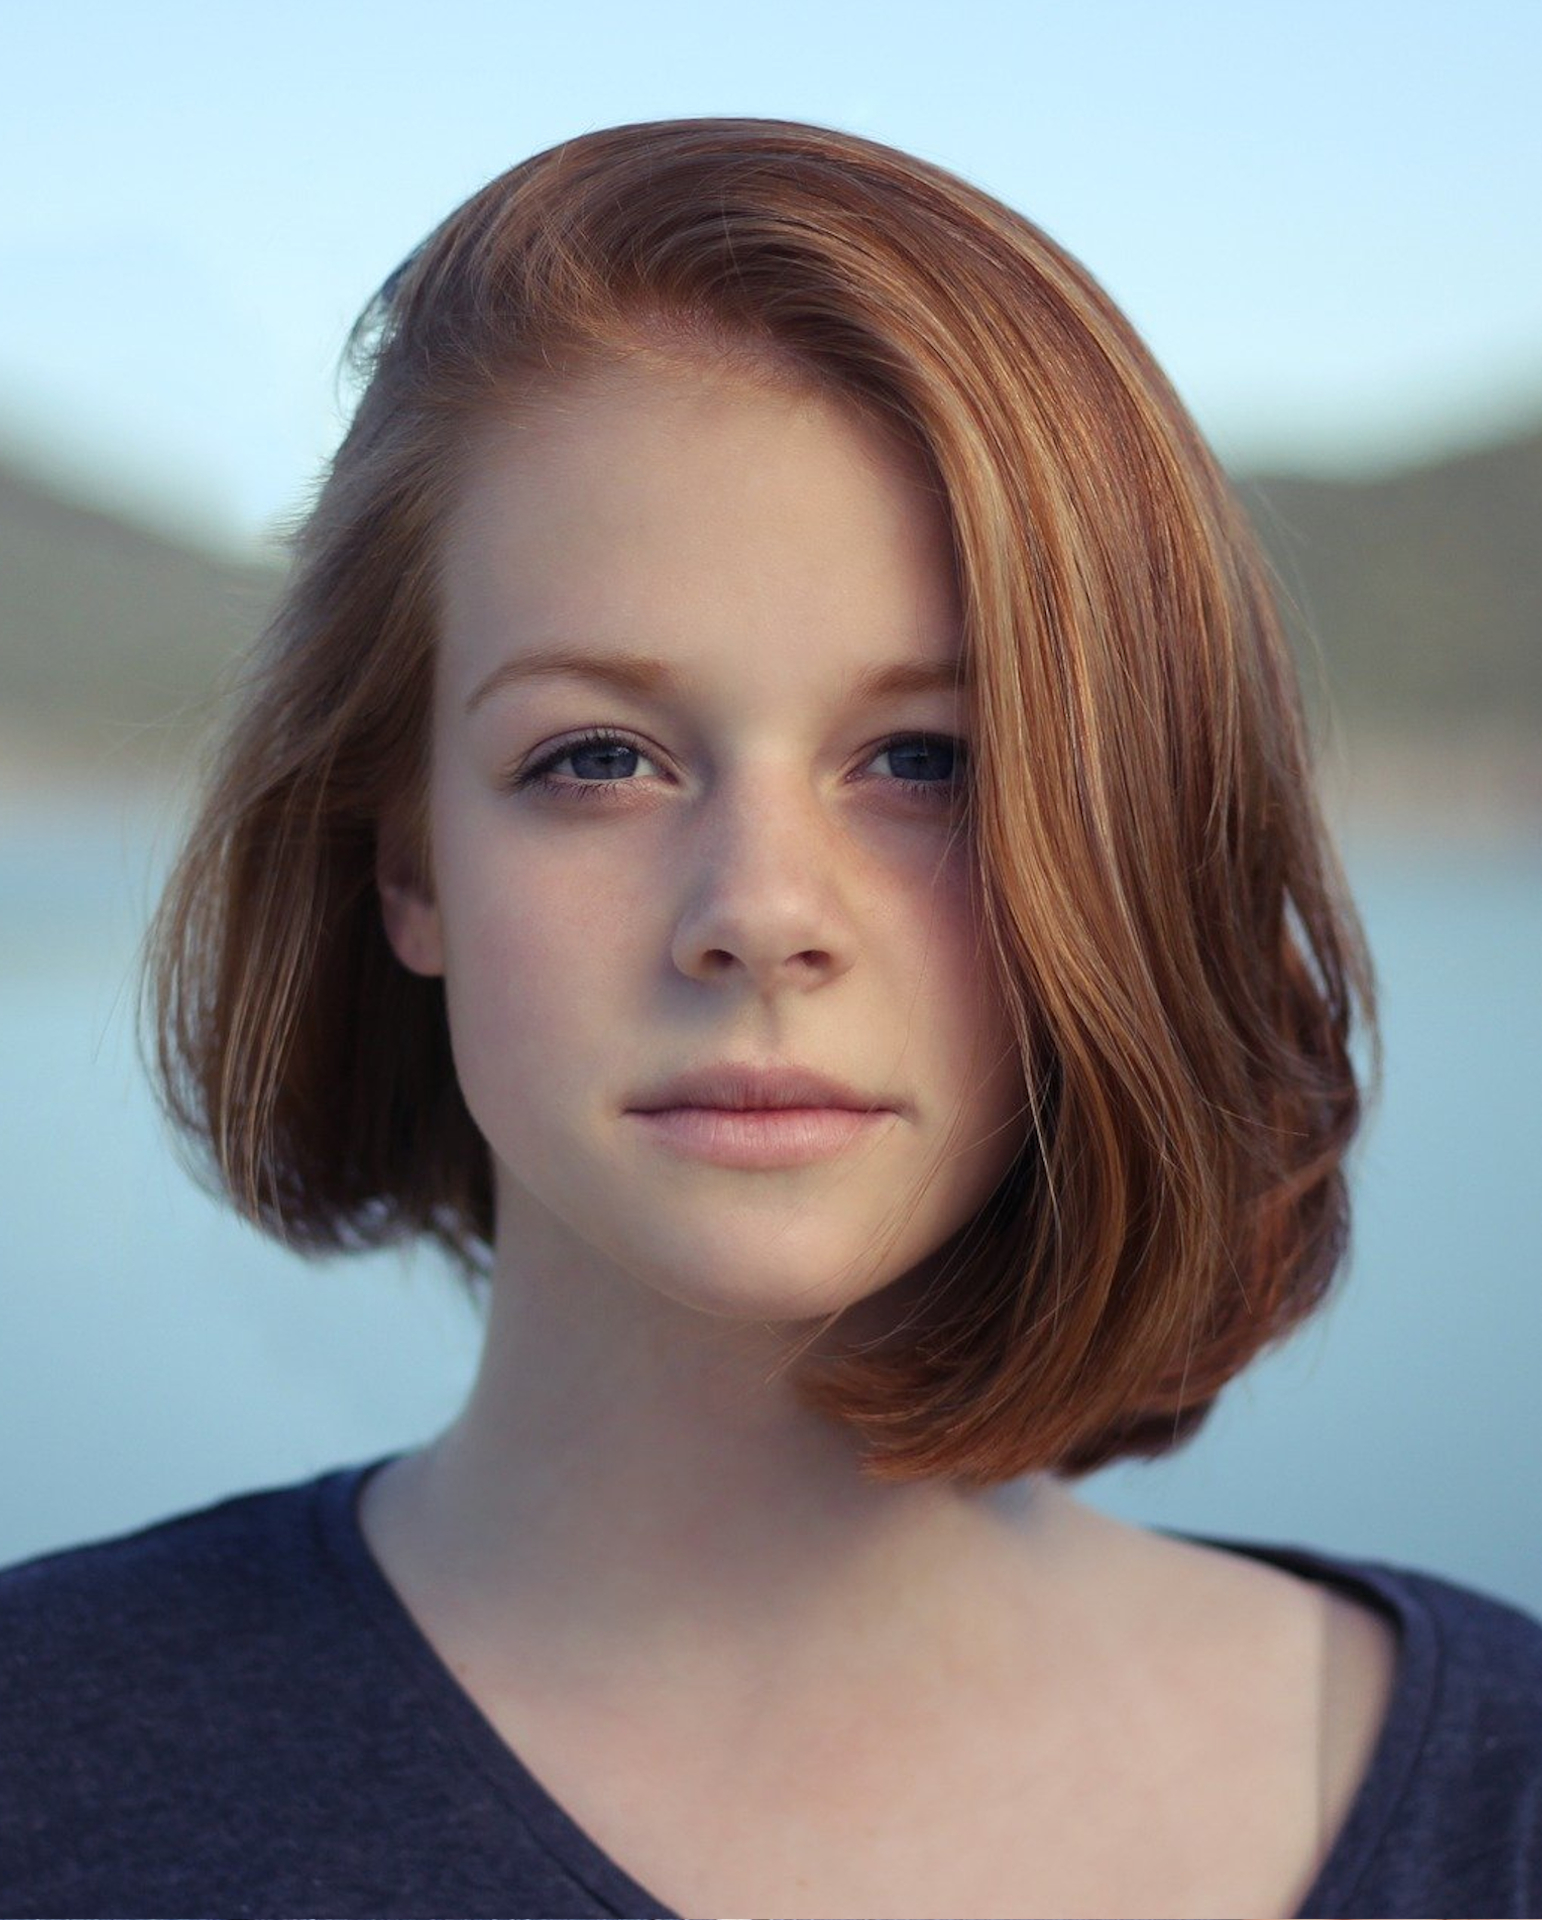
\includegraphics[scale=0.06]{figuras/personas/girl-919048_1920.jpg}
Fonte: Pixabay\tablefootnote{https://pixabay.com/photos/girl-portrait-hairstyle-redhead-919048/}
\end{center} 

&

\textbf{Nome: }  Natália Figueiredo

\textbf{Idade:} 23 anos

\textbf{Ocupação:} Estudante de Engenharia de Software na UnB, Faculdade do Gama.

\\ \hline


\multicolumn{2}{|c|}{\textbf{Descrição}} \\ \hline
\multicolumn{2}{|p{15cm}|}{
    \begin{tabular}[c]{@{}l@{}}\\
        Nunca joguei jogos educacionais, pois não conheci nenhum que tinha o propósito de\\ ensinar o que eu desejava. No caso se eu encontrasse um jogo o qual eu pudesse aprender\\ um conteúdo novo e pudesse revisá-lo quando necessário seria interessante. Estou fazendo\\ a disciplina de IHC e desejaria utilizar um jogo que me ajudasse a aprender o conteúdo,\\ pois não tenho muito conhecimento em relação a elaboração de design de interfaces e o\\ pouco que tenho foi somente a partir da disciplina de IHC.\\
        \\
        Geralmente quando vou estudar ou sanar alguma dúvida que tenho sobre o conteúdo eu\\ pesquiso na internet. Em ocasiões bem específicas eu assisto vídeo aulas e também\\ utilizo do material disponibilizado pelo professor. \\
        \\
        Acho que um jogo para se estudar teria de ter um \textbf{design simples}, uma lógica de jogo e\\ \textbf{regras fáceis} de se lembrar. O jogo não deveria ser muito \textbf{difícil}, sendo que o objetivo\\ com ele é aprender. Talvez \textbf{recompensas} e \textbf{mensagens} evidenciando meu progresso\\ seriam interessantes.\\
        \\
        Ao jogar, espero encontrar \textbf{desafios} não muito difíceis, mas que despertem minha\\ \textbf{atenção}. Seria bom, perceber logo de início que o jogo traz um \textbf{conteúdo relevante} e \\que vou \textbf{conseguir aprendê-lo}. E por fim não seria nada ruim sentir \textbf{prazer} em \\aprender e ainda me \textbf{divertir}.\\
        \\
    \end{tabular}
} \\ \hline
\end{tabular}
\end{table}
\newpage


\begin{table}[htbp]
\centering
\caption{Anti Persona}
\label{tab:Table_persona4}
\small
\begin{tabular}{| m{0.25\textwidth} m{0.65\textwidth}|}
\hline \multicolumn{2}{|c|}{\textbf{Identidade}} \\ \hline
& \\

\begin{center} 
\includegraphics[scale=0.06]{figuras/personas/man-1209494_1920.jpg} \end{center} 

&

\textbf{Nome: }  Rafael Medeiros

\textbf{Idade:} 28 anos

\textbf{Ocupação:} Estudante de Educação Física na UnB, campus Darcy Ribeiro.

\\ \hline


\multicolumn{2}{|c|}{\textbf{Descrição}} \\ \hline
\multicolumn{2}{|p{15cm}|}{
        Não tenho o costume de usar jogos educacionais, devo ter jogado um alguma vez na vida, mas não me interessei muito e rapidamente o jogo se tornou monótono. Gosto de jogar futebol e basquetebol. Em relação ao conhecimento acadêmico, me concentro apenas nas disciplinas do meu curso.
        
        Quando vou estudar ou sanar alguma dúvida que tenho sobre o conteúdo eu utilizo todos os recursos possíveis, priorizando o que for mais prático e objetivo. Geralmente eu tiro dúvidas com colegas que já fizeram a disciplina e colegas que cursam a disciplina comigo. Somente se realmente necessário que vou tirar as dúvidas com os monitores ou professor da matéria. Os requisitos do jogo que me levariam a usá-lo são: 
        
        \begin{itemize}
            \item um design atraente e consistente; 
            \item o jogo ser fácil de aprender a jogar e fácil de se jogar, com regras claras; 
            \item um bom uso de fontes e cores; 
            \item  o jogo ter uma história que me envolvesse seria algo interessante;
            \item que o jogo ofereçam feedbacks relevantes;
            \item pontos e recompensas;
            \item gosto de jogos que promovam interação com outros jogadores, como por exemplo ranking dos jogadores.
        \end{itemize}
        
        Ao usar um jogo eu espero aprender o conteúdo ali apresentado, espero que seja algo desafiador, divertido e satisfatório aprender jogando. Jogos que prendem minha atenção e me envolvem para  aprender o conteúdo são bem relevantes, ainda mais se eu conseguir perceber a importância do conteúdo que estou aprendendo.

       } \\ \hline
\end{tabular}
\end{table}

\chapter{Protótipo de Papel}
\label{ap:proto_papel}

{\color{textmodified}
Neste capítulo estão apresentadas as telas do protótipo de baixa fidelidade, a estrutura de avaliação do protótipo e o relato dos resultados da avaliação. Para a produção deste protótipo de baixa fidelidade, foi utilizado a prototipação em papel.
}

\section{Telas do protótipo de papel}

{\color{textadded}
A prototipagem em papel é um método para avaliar a usabilidade de um design de IHC representado em papel \cite{barbosa_silva}. Por ser feita em papel é uma maneira rápida e barata de identificar problemas na usabilidade \cite{barbosa_silva}, assim tendo um maior foco na usabilidade do que no design final do software.

Nas Figuras \ref{Fig:proto1.png}, \ref{Fig:proto2.png} e \ref{Fig:proto3.png} são apresentadas algumas das principais telas do protótipo de papel. Este protótipo de papel é a versão final após refinamentos realizados durante as validações do protótipo (Seção \ref{sec:aval_prototipo_papel}).

Na Figura \ref{Fig:menu.png} é apresentado o menu principal do jogo, onde dá acesso as telas de: ambiente de resumos, Figura \ref{Fig:resumos.png}; início do jogo, Figura \ref{Fig:fases.png}; e ambiente de recompensas, Figuras \ref{Fig:recomp_persona.png} e \ref{Fig:recomp_medalhas.png}.

Ao iniciar o jogo é visualizado as fases e etapas disponíveis ao usuário, como apresentada na Figura \ref{Fig:fases.png}. Através dela é possível que o jogador inicie uma partida, e ao iniciar é necessário confirmar esta ação, como apresentado na Figura \ref{Fig:partida_confirm.png}.

Dentro de uma partida são realizadas perguntas referente ao tema da fase e etapa. Estas perguntas são dividas em verdadeiro ou falso e múltipla escolha, Figura \ref{Fig:question_tf.png} e \ref{Fig:question_me.png}, respectivamente. Ao selecionar uma resposta é necessário que o usuário confirme a opção selecionada, Figura \ref{Fig:question_confirm.png}. Após a confirmação será apresentado o \textit{feedback} da resposta, podendo ser um erro ou acerto. No caso de erro é apresentada uma mensagem de erro e uma explicação da resposta correta, Figura \ref{Fig:question_erro.png}. Já no caso de acerto é apresentada uma mensagem de congratulação e possivelmente uma recompensa, Figuras \ref{Fig:question_acerto.png} e \ref{Fig:question_recomp.png}.

O protótipo de papel interativo foi desenvolvido através da plataforma do marvelapp\footnote{https://marvelapp.com} e pode ser acesso pelo link \url{https://marvelapp.com/prototype/9gh9jg7/screen/78409022}.

}

\newpage
\begin{figure}[htbp]
	\centering
    \subfigure[\textcolor{textmodified}{Menu Principal}]{
        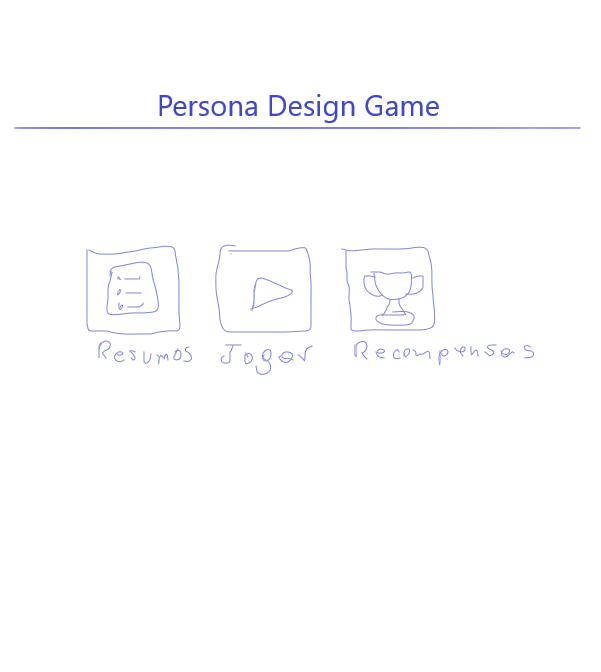
\includegraphics[keepaspectratio=true,scale=0.4]{figuras/prototype/proto1.png}
        \label{Fig:menu.png}
    }
    \quad
    \subfigure[\textcolor{textmodified}{Ambiente Resumos}]{
        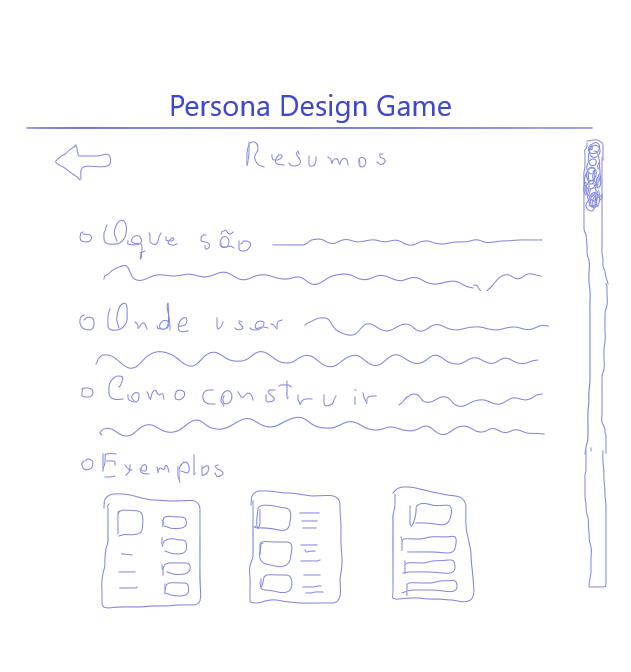
\includegraphics[keepaspectratio=true,scale=0.4]{figuras/prototype/proto2.png}
        \label{Fig:resumos.png}
    }
    \quad
    \subfigure[\textcolor{textmodified}{Ambiente Recompensas - Persona}]{
        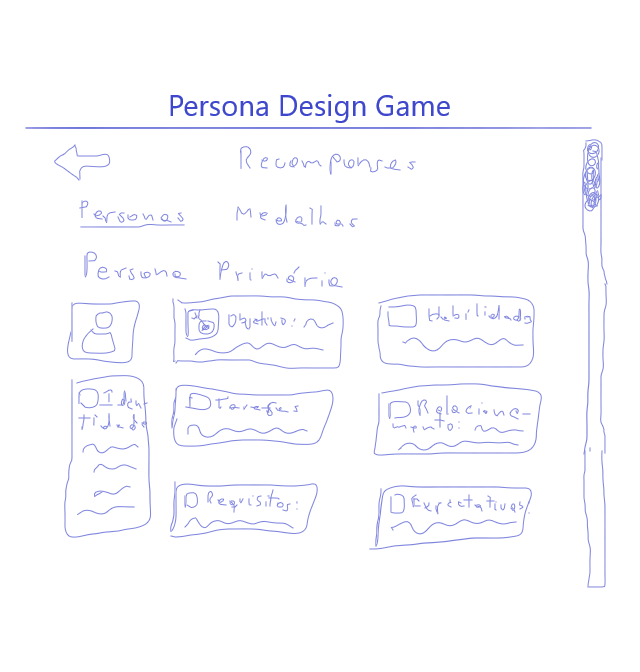
\includegraphics[keepaspectratio=true,scale=0.4]{figuras/prototype/proto3.png}
        \label{Fig:recomp_persona.png}
    }
    \quad
    \subfigure[\textcolor{textmodified}{Ambiente Recompensas - Medalhas}]{
        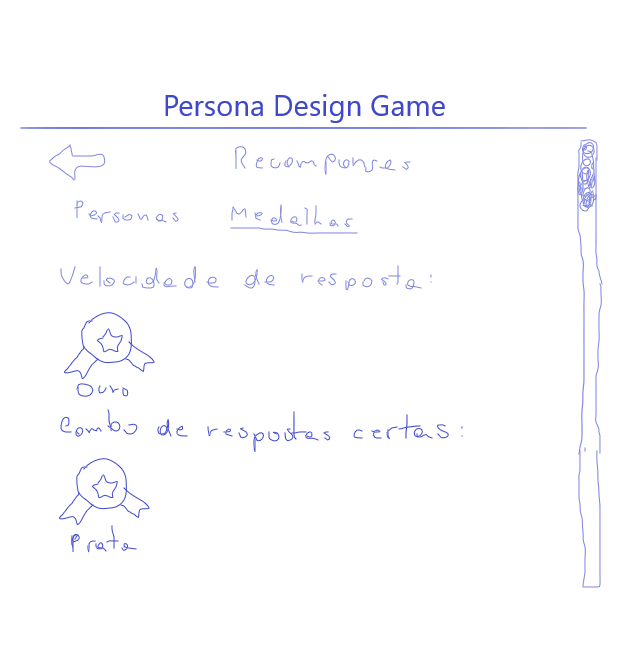
\includegraphics[keepaspectratio=true,scale=0.4]{figuras/prototype/proto4.png}
        \label{Fig:recomp_medalhas.png}
    }
    
	\caption{\textcolor{textmodified}{Telas do Protótipo de Papel 1 - Próprios Autores}}
	\label{Fig:proto1.png}
\end{figure}

\newpage
\begin{figure}[htbp]
	\centering
    \subfigure[\textcolor{textmodified}{Fases}]{
        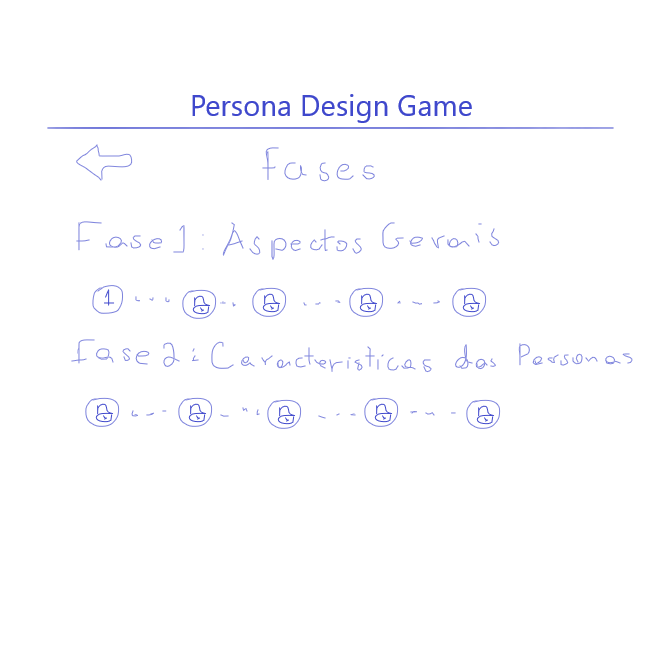
\includegraphics[keepaspectratio=true,scale=0.37]{figuras/prototype/proto5.png}
        \label{Fig:fases.png}
    }
    \quad
    \subfigure[\textcolor{textmodified}{Confirmar Iniciar Etapa}]{
        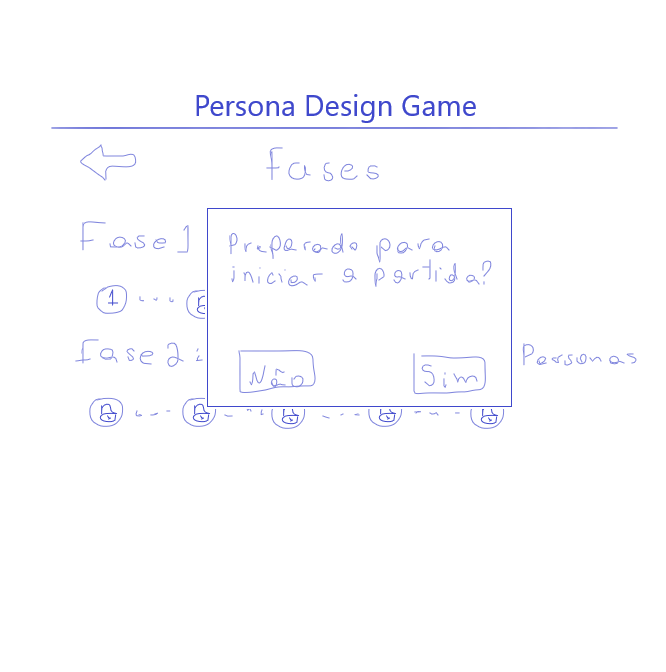
\includegraphics[keepaspectratio=true,scale=0.37]{figuras/prototype/proto6.png}
        \label{Fig:partida_confirm.png}
    }
    \quad
    \subfigure[\textcolor{textmodified}{Questão - Verdadeiro ou Falso}]{
        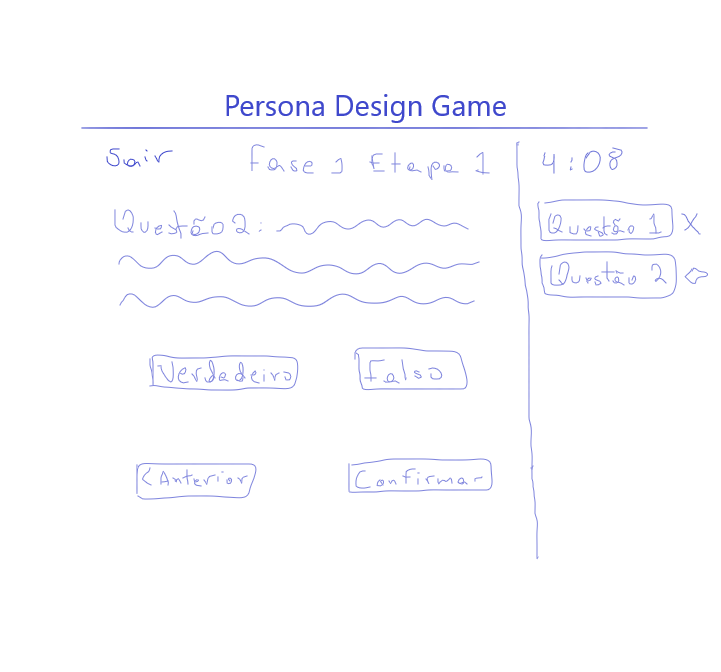
\includegraphics[keepaspectratio=true,scale=0.37]{figuras/prototype/proto10.png}
        \label{Fig:question_tf.png}
    }
    \quad
    \subfigure[\textcolor{textmodified}{Questão - Múltipla Escolha}]{
        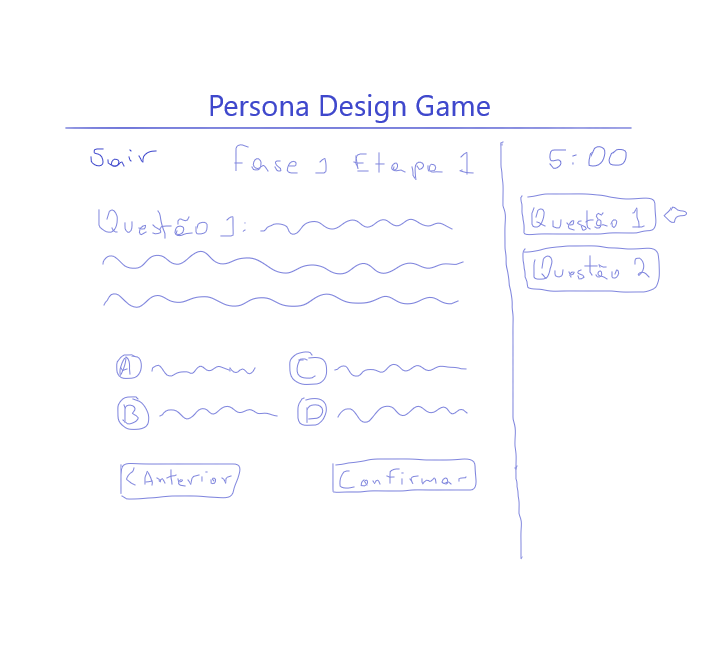
\includegraphics[keepaspectratio=true,scale=0.37]{figuras/prototype/proto7.png}
        \label{Fig:question_me.png}
    }
    
	\caption{\textcolor{textmodified}{Telas do Protótipo de Papel 2 - Próprios Autores}}
	\label{Fig:proto2.png}
\end{figure}

\newpage
\begin{figure}[htbp]
	\centering
    \subfigure[\textcolor{textmodified}{Questão - Confirmar Resposta}]{
        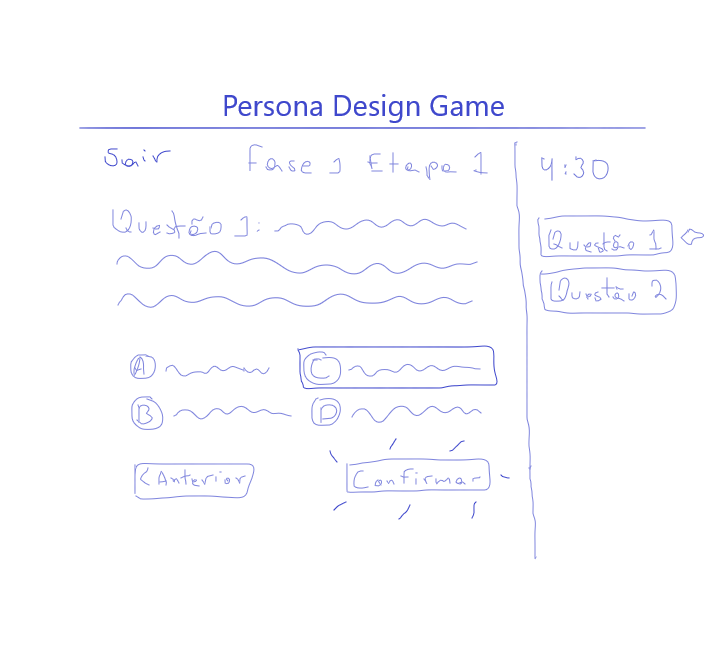
\includegraphics[keepaspectratio=true,scale=0.37]{figuras/prototype/proto8.png}
        \label{Fig:question_confirm.png}
    }
    \quad
    \subfigure[\textcolor{textmodified}{Questão - Erro}]{
        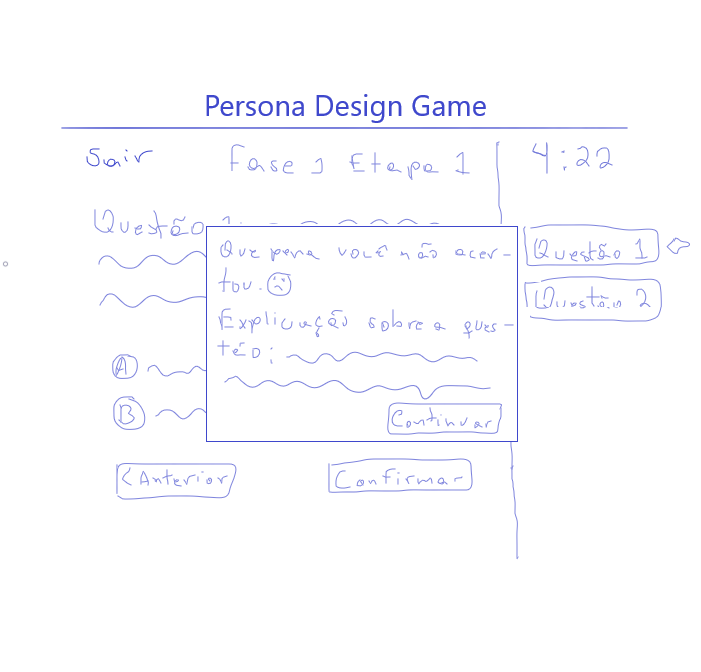
\includegraphics[keepaspectratio=true,scale=0.37]{figuras/prototype/proto9.png}
        \label{Fig:question_erro.png}
    }
    \quad
	\subfigure[\textcolor{textmodified}{Questão - Acerto}]{
        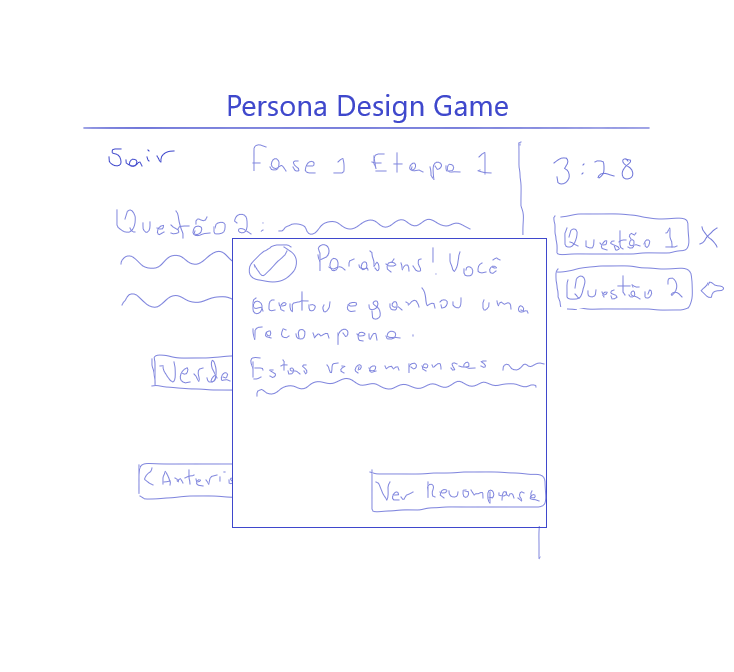
\includegraphics[keepaspectratio=true,scale=0.37]{figuras/prototype/proto11.png}
        \label{Fig:question_acerto.png}
    }
    \quad
    \subfigure[\textcolor{textmodified}{Questão - Recompensa}]{
        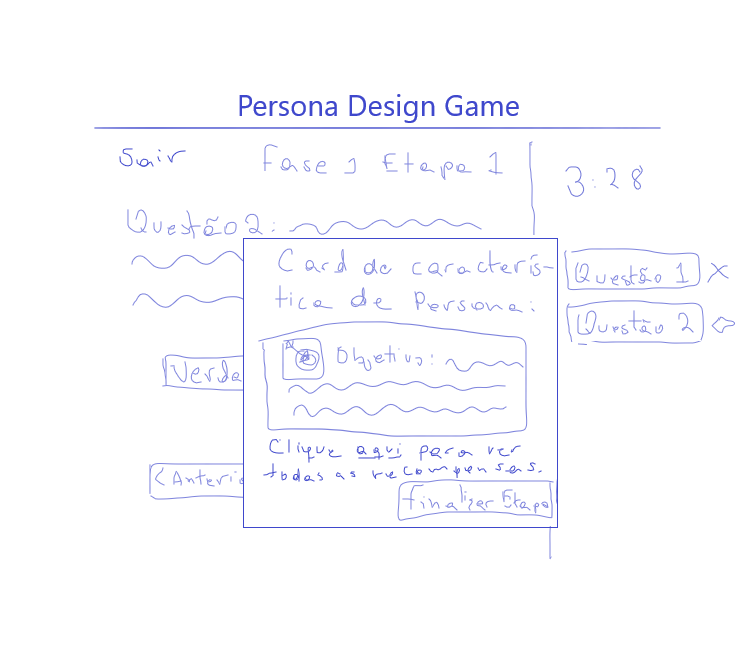
\includegraphics[keepaspectratio=true,scale=0.37]{figuras/prototype/proto12.png}
        \label{Fig:question_recomp.png}
    }
	\caption{\textcolor{textmodified}{Telas do Protótipo de Papel 3 - Próprios Autores}}
	\label{Fig:proto3.png}
\end{figure}

\newpage
\section{Avaliação do protótipo de papel}
\label{sec:aval_prototipo_papel}

{\color{textadded}
Para a avaliação do protótipo de papel, foi utilizado o planejamento das atividades citadas por \citeonline{barbosa_silva}. Estas atividades são definidas na Tabela \ref{tab:aval-prot-papel}.
}

\begin{table}[h!]
\centering
\caption{Atividades da avaliação do protótipo de papel \cite[p. 359]{barbosa_silva}}
\begin{tabular}{|p{5cm}|p{10.5cm}|}
\hline
{\color{textadded} \textbf{Atividade}}           & {\color{textadded} \textbf{Tarefas}}                                                                            \\ \hline
{\color{textadded}Preparação }                             & {\color{textadded} Definir tarefa para os participantes executarem}                                             \\ \cline{2-2} 
{\color{textadded} }                             & {\color{textadded} Definir o perfil dos participantes e recrutá-los}                                            \\ \cline{2-2} 
{\color{textadded} }                             & {\color{textadded} Criar protótipo de papel da interface para executar as tarefas}                              \\ \cline{2-2} 
 & {\color{textadded} Executar um teste piloto}   \\ \hline
{\color{textadded} Coleta de Dados e Interpretação}   & {\color{textadded} Cada usuário deve executar as tarefas propostas interagindo com o protótipo de papel, mediado pelo avaliador.}       \\ \cline{2-2} 
   & {\color{textadded} Avaliador deve listar os problemas encontrados e refinar o protótipo de papel para eliminar problemas mais simples.} \\ \hline
{\color{textadded} Consolidação dos Resultados}& {\color{textadded}Priorizar a correção dos problemas não resolvidos.}                                                                  \\ \cline{2-2} 
       & {\color{textadded}Sugerir correção.}                                                                                                   \\ \hline
{\color{textadded}Relato dos Resultados}                               & {\color{textadded}Relatar os problemas encontrados e sugestões de correção.}                                                           \\ \hline
\end{tabular}
\label{tab:aval-prot-papel}
\end{table}

{\color{textadded}
De acordo com a Tabela \ref{tab:aval-prot-papel}, as atividades de preparação, coleta de dados e interpretação, consolidação dos resultados e relato dos resultados são as etapas seguidas para que seja feito a avaliação de um protótipo de papel. Cada atividade é dividida em uma ou mais tarefas a serem executadas. Nas subseções a seguir é apresentado o resultado da execução dessas atividades.

\subsection{Preparação}

As tarefas a serem executadas pelos participantes foram definidas de forma a simular o uso esperado de um jogador comum, abrangendo os principais requisitos do jogo. É necessário a execução das tarefas em ordem crescente, para que o usuário siga um fluxo lógico do jogo.

Tarefas:
\begin{enumerate}   
    \item Inicie o jogo.
    \item Comece a etapa 1 da fase 1.
    \item Responda a primeira questão de múltipla escolha com a opção C.
    \item Responda a segunda questão de verdadeiro ou falso como falso.
    \item Após receber uma recompensa, acesse o ambiente de recompensas.
\end{enumerate}

De acordo com \citeonline{nielsen2000}, com cinco participantes já é possível cobrir cerca de 80\% dos problemas de usabilidade de um software. A adição de mais participantes faz com que seja observado muitos problemas já conhecidos, assim perdendo muito tempo com observações repetitivas. Com isso foi definido recrutar cinco participantes para cada teste de usabilidade a ser realizado.


Definido a quantidade de participantes, foram utilizadas as três personas do projeto e solicitada a participação de dois estudantes de engenharia de software. A utilização das personas nesta etapa facilita a encontrar o que precisa ser melhorado dentro do fluxo do jogo, visto que a persona possui o perfil dos usuários finais. Já os estudantes de engenharia de software podem também dar um feedback mais técnico, visto que é estudado IHC no curso.

Com o objetivo de descobrir se os usuários conseguem completar o fluxo de iniciar o jogo e responder perguntas de uma fase, foi levantado tarefas que visam abranger todo esse fluxo principal. Dando um maior foco para o uso esperado das personas definidas do projeto. Com isso as tarefas englobam o acerto e erro de uma questão, para que seja possível validar o feedback do jogo ao usuário e também a conquista de uma recompensa, podendo observar a reação do usuário ao recebe-la.

\subsection{Relato dos Resultados}

A última atividade a ser executada na avaliação do protótipo de papel (Tabela \ref{tab:aval-prot-papel}) é composta pela tarefa de relatar os problemas encontrados durante o validação do protótipo e sugestões de correção destes problemas. Estes problemas foram anotados e corrigidos posteriormente.

Após a finalização de cada validação do protótipo com um participante, foram realizadas perguntas referentes as metas de experiência do jogador (Tabela \ref{tab:Table_px}). Para cada uma das metas, foi pedido uma nota entre 0 e 4, onde 0 representa a pior nota e 4 representa a melhor nota.

Foram realizadas duas validações do protótipo de papel, nas sub-subseções \ref{sssec:val-prot-papel-1} e \ref{sssec:val-prot-papel-2} são apresentados duas tabelas para cada validação realizada, uma das tabelas apresentam os problemas encontrados com suas sugestões de correção e a outra as notas dadas pelos participantes para cada meta de experiência do jogador.

O feedback dos participantes através das notas de meta de experiência para uma validação de um protótipo de baixa-fidelidade pode não ser muito preciso por não possuir toda a experiência de um jogo funcional, com atenção ao design e textos relevantes. Entretanto, é muito importante a constante avaliação das metas de experiência do jogador \cite{Fullerton_2008}, visto que estas metas de experiência são objetivos a serem atingido durante o uso de um usuário.

\subsubsection{Primeira iteração de validação do protótipo} \label{sssec:val-prot-papel-1}

Na Tabela \ref{tab:Table_resultados_prototipo_de_papel_1}, são apresentados os problemas encontrados e sugestões de correção. Foram aplicadas todas as sugestões de correção no protótipo para os problemas elencados.

\begin{table}[htbp]
\centering
\caption{\textcolor{textadded}{Problemas da primeira validação do protótipo de papel}}
\begin{tabular}{|p{7.5cm}|p{7.5cm}|}
\hline
\textbf{\textcolor{textadded}{Problema}}                       & \textbf{\textcolor{textadded}{Sugestão de correção}} \\ \hline
\textcolor{textadded}{Modal de certo e errado não possui botão para ir para a próxima questão} & \textcolor{textadded}{Adicionar botão para continuar a responder as perguntas}      \\ \hline
\textcolor{textadded}{Modal de recompensa não possui botão para fechar e ir para próxima questão} & \textcolor{textadded}{Adicionar botão para continuar a responder as perguntas}      \\ \hline
\textcolor{textadded}{Ao receber uma recompensa o usuário não entende o significado da recompensa} & \textcolor{textadded}{Adicionar explicação sobre as recompensas quando o usuário receber sua primeira recompensa}       \\ \hline
\textcolor{textadded}{Ao clicar em sair de uma partida, o jogo não pede uma confirmação da ação} & \textcolor{textadded}{Adicionar modal de confirmação ao clicar para sair de uma partida e explicar sobre a perca do progresso da fase}    \\ \hline
\textcolor{textadded}{Ao clicar para visualizar uma questão anterior, não existe um botão para ir para a próxima questão} & \textcolor{textadded}{Adicionar botão para próxima questão}    \\ \hline
\textcolor{textadded}{O nome ambiente de personas pode ser pouco intuitivo para que o usuário saiba onde estão suas recompensas} & \textcolor{textadded}{Adicionar ícone que se assemelha a recompensas}  \\ \hline
\textcolor{textadded}{Ao responder perguntas de uma fase, não é apresentado um histórico das perguntas anteriores} & \textcolor{textadded}{Apresentar progresso de respostas de perguntas anteriores e perguntas futuras}   \\ \hline
\textcolor{textadded}{O significado das recompensas que são armazenadas no ambiente de personas não está muito claro para o usuário} & \textcolor{textadded}{Apresentar uma breve explicação sobre o significado das recompensas dentro do ambiente de personas}   \\ \hline
\end{tabular}
\label{tab:Table_resultados_prototipo_de_papel_1}
\end{table}

Na Tabela \ref{tab:notas-metas-exp-1}, são apresentadas as notas dadas pelos participantes, referentes as metas de experiência do jogador (Tabela \ref{tab:Table_px}). As colunas U1, U2 representam os dois usuários participantes. As colunas P1, P2 e P3 representam a persona primária, secundária e suplementar, respectivamente.

\begin{table}[htbp]
\centering
\caption{\textcolor{textadded}{Notas de experiência da primeira validação do protótipo de papel}}
\begin{tabular}{|p{5cm}|r|r|r|r|r|r|r|}
\hline
\textcolor{textadded}{\textbf{Metas de Experiência}} & \textcolor{textadded}{\textbf{U1}} & \textcolor{textadded}{\textbf{U2}} & \textcolor{textadded}{\textbf{P1}} & \textcolor{textadded}{\textbf{P2}} & \textcolor{textadded}{\textbf{P3}} & \textcolor{textadded}{\textbf{Score}} & \textcolor{textadded}{\textbf{Porcentagem Total}}     \\ \hline
\textcolor{textadded}{Satisfação} & \textcolor{textadded}{3} & \textcolor{textadded}{3} & \textcolor{textadded}{4} & \textcolor{textadded}{3} & \textcolor{textadded}{2} & \textcolor{textadded}{15} & \textcolor{textadded}{75,00\%}         \\ \hline
\textcolor{textadded}{Confiança} & \textcolor{textadded}{4} & \textcolor{textadded}{4} & \textcolor{textadded}{4} & \textcolor{textadded}{3} & \textcolor{textadded}{4} & \textcolor{textadded}{19} & \textcolor{textadded}{95,00\%}          \\ \hline
\textcolor{textadded}{Relevância} & \textcolor{textadded}{0} & \textcolor{textadded}{4} & \textcolor{textadded}{2} & \textcolor{textadded}{3} & \textcolor{textadded}{3} & \textcolor{textadded}{12} & \textcolor{textadded}{60,00\%}         \\ \hline
\textcolor{textadded}{Atenção Focada} & \textcolor{textadded}{3} & \textcolor{textadded}{4} & \textcolor{textadded}{2} & \textcolor{textadded}{2} & \textcolor{textadded}{2} & \textcolor{textadded}{13} & \textcolor{textadded}{65,00\%}     \\ \hline
\textcolor{textadded}{Desafio} & \textcolor{textadded}{2} & \textcolor{textadded}{2} & \textcolor{textadded}{2} & \textcolor{textadded}{1} & \textcolor{textadded}{1} & \textcolor{textadded}{8} & \textcolor{textadded}{40,00\%}             \\ \hline
\textcolor{textadded}{Diversão} & \textcolor{textadded}{2} & \textcolor{textadded}{1} & \textcolor{textadded}{2} & \textcolor{textadded}{2} & \textcolor{textadded}{2} & \textcolor{textadded}{9} & \textcolor{textadded}{45,00\%}            \\ \hline
\end{tabular}
\label{tab:notas-metas-exp-1}
\end{table}

\newpage

Após esta validação do protótipo de papel, foram notados alguns problemas de usabilidade, além de uma baixa nota na experiência do jogador em desafio e diversão. Estes problemas encontrados foram corrigidos e com isso, foi realizada uma segunda validação do protótipo apresentada a seguir.

\subsubsection{Segunda iteração de validação do protótipo} \label{sssec:val-prot-papel-2}

Com o objetivo de melhorar a experiência do jogador no quesito de desafio e diversão, foi realizado um \textit{Brainstorming}. Com as ideias geradas, foram adicionados novos requisitos referente a novas recompensas (RF17 e RF18), tempo limite para cada etapa (RF13) e quantidade mínima de acerto para completar uma etapa (RF12). Os requisitos referentes a estas novas funcionalidades podem ser observados na Tabela \ref{tab:Table_rf}.

Na Tabela \ref{tab:Table_resultados_prototipo_de_papel_2}, são apresentados os problemas encontrados e sugestões de correção. Foram aplicadas todas as sugestões de correção no protótipo para os problemas elencados.

\begin{table}[htbp]
\centering
\caption{\textcolor{textadded}{Problemas da segunda validação do protótipo de papel}}
\begin{tabular}{|p{7.5cm}|p{7.5cm}|}
\hline
\textbf{\textcolor{textadded}{Problema}}                       & \textbf{\textcolor{textadded}{Sugestão de correção}} \\ \hline
\textcolor{textadded}{O número da etapa não é evidenciado no menu de fases} & \textcolor{textadded}{Adicionar número da etapa no circulo que representa a etapa}      \\ \hline
\textcolor{textadded}{Botão de confirmar para entrar em uma fase na esquerda, e cancelar na direita, fugindo do padrão} & \textcolor{textadded}{Padronizar as opções de cancelar/confirmar, com o cancelar na esquerda e confirmar na direita}      \\ \hline
\textcolor{textadded}{Ao receber uma recompensa, o usuário depende da memória para acessar a galeria de recompensas} & \textcolor{textadded}{Adicionar botão para ir a galeria de recompensas ao receber uma recompensa}      \\ \hline
\textcolor{textadded}{Botão de sair de uma etapa pouco intuitivo} & \textcolor{textadded}{Mudar o ícone do botão de sair para o texto 'sair'}      \\ \hline
\textcolor{textadded}{Ao selecionar uma opção de resposta, não ficou intuitivo que deveria confirmar a resposta} & \textcolor{textadded}{Adicionar realce no botão de confirmar resposta, quando selecionado uma opção de resposta}      \\ \hline
\end{tabular}
\label{tab:Table_resultados_prototipo_de_papel_2}
\end{table}

Na Tabela \ref{tab:notas-metas-exp-2}, são apresentadas as notas dadas pelos participantes, referentes as metas de experiência do jogador (Tabela \ref{tab:Table_px}). As colunas U1, U2 representam os 2 (dois) usuários participantes. As colunas P1, P2 e P3 representam a persona primária, secundária e suplementar, respectivamente.

\begin{table}[htbp]
\centering
\caption{\textcolor{textadded}{Notas de experiência da primeira validação do protótipo de papel}}
\begin{tabular}{|p{5cm}|r|r|r|r|r|r|r|}
\hline
\textcolor{textadded}{\textbf{Metas de Experiência}} & \textcolor{textadded}{\textbf{U1}} & \textcolor{textadded}{\textbf{U2}} & \textcolor{textadded}{\textbf{P1}} & \textcolor{textadded}{\textbf{P2}} & \textcolor{textadded}{\textbf{P3}} & \textcolor{textadded}{\textbf{Score}} & \textcolor{textadded}{\textbf{Porcentagem Total}}     \\ \hline
\textcolor{textadded}{Satisfação} & \textcolor{textadded}{2} & \textcolor{textadded}{4} & \textcolor{textadded}{4} & \textcolor{textadded}{4} & \textcolor{textadded}{4} & \textcolor{textadded}{18} & \textcolor{textadded}{90,00\%}         \\ \hline
\textcolor{textadded}{Confiança} & \textcolor{textadded}{3} & \textcolor{textadded}{4} & \textcolor{textadded}{4} & \textcolor{textadded}{4} & \textcolor{textadded}{4} & \textcolor{textadded}{19} & \textcolor{textadded}{95,00\%}          \\ \hline
\textcolor{textadded}{Relevância} & \textcolor{textadded}{3} & \textcolor{textadded}{4} & \textcolor{textadded}{3} & \textcolor{textadded}{4} & \textcolor{textadded}{4} & \textcolor{textadded}{18} & \textcolor{textadded}{90,00\%}         \\ \hline
\textcolor{textadded}{Atenção Focada} & \textcolor{textadded}{4} & \textcolor{textadded}{4} & \textcolor{textadded}{4} & \textcolor{textadded}{4} & \textcolor{textadded}{4} & \textcolor{textadded}{20} & \textcolor{textadded}{100,00\%}     \\ \hline
\textcolor{textadded}{Desafio} & \textcolor{textadded}{2} & \textcolor{textadded}{4} & \textcolor{textadded}{3} & \textcolor{textadded}{3} & \textcolor{textadded}{3} & \textcolor{textadded}{15} & \textcolor{textadded}{75,00\%}             \\ \hline
\textcolor{textadded}{Diversão} & \textcolor{textadded}{2} & \textcolor{textadded}{3} & \textcolor{textadded}{3} & \textcolor{textadded}{3} & \textcolor{textadded}{2} & \textcolor{textadded}{13} & \textcolor{textadded}{65,00\%}            \\ \hline
\end{tabular}
\label{tab:notas-metas-exp-2}
\end{table}

Como é possível observar na Tabela \ref{tab:notas-metas-exp-2}, houve um melhoria nas experiências do jogador, comparado a primeira validação (Tabela \ref{tab:notas-metas-exp-1}). Esta melhoria ficou de acordo com o que era esperado, visto que foi adicionado novos requisitos com o intuito de melhorar estas experiências. Para a definição de uma nota desejada foi levado como base as características da persona primária do projeto (Tabela \ref{tab:Table_persona1}).

}

\end{apendicesenv}